\documentclass{note}
\usepackage[cpp,table]{mypackage}
\usepackage{footnote}
\makesavenoteenv{tabular}

\renewcommand{\thefootnote}{\fnsymbol{footnote}}

\title{数字图像处理笔记}
\author{陈鸿峥}
\date{{\builddatemonth\today}\protect\footnote{\text{Build \builddate\today}}} % protect!

\begin{document}

\maketitle
\renewcommand{\thefootnote}{\arabic{footnote}}
\setcounter{footnote}{0}

\setcounter{tocdepth}{2}%设置深度
\tableofcontents

\bigskip\bigskip

% !TEX root = main.tex

\section{计算机系统概述}
\subsection{计算模型}
\begin{itemize}
	\item 图灵机(1936)
	\item 冯诺依曼体系结构(1945)\footnote{非冯诺依曼体系结构:并行计算、量子计算、生物计算} --- 存储程序原理(\textbf{运算器}为中心)\\
	计算机采用\textbf{二进制}表示机器指令和数据,按照程序指令\textbf{顺序}执行
\begin{center}
\begin{tikzcd}
& & \text{存储器}\arrow{d} & & \\
\quad\arrow{r} & \text{输入设备}\arrow{r} & \text{运算器}\arrow{r}\arrow{d}\arrow{u} & \text{输出设备}\arrow{r} & \quad\\
& & \text{控制器}\arrow{u}\arrow{lu}\arrow{ru}\arrow[bend left]{uu} & &
\end{tikzcd}
\end{center}
而现在由于计算不是瓶颈,存储访问成为了瓶颈,故现代微机以\textbf{存储器}为中心
\begin{center}
\begin{tikzcd}
& & \text{运算器}\arrow{d} & & \\
\quad\arrow{r} & \text{输入设备}\arrow{r} & \text{存储器}\arrow{r}\arrow{d}\arrow{u} & \text{输出设备}\arrow{r} & \quad\\
& & \text{控制器}\arrow{u}\arrow{lu}\arrow{ru}\arrow[bend left]{uu} & &
\end{tikzcd}
\end{center}
\end{itemize}
[运算器、控制器](CPU)、存储器为计算机的核心,合称主机;外围设备,简称外设,指除主机外的其他设备,包括IO设备、外存等

计算机中的信息仍用二进制表示的原因:由物理器件性能决定
\begin{itemize}
	\item 二进制只有两种状态,容易找到具有2个稳定状态并且状态转换容易控制的物理器件(数字电路)
	\item 二进制编码运算规则简单
	\item 二进制的0、1与二值逻辑一致,容易实现逻辑运算
\end{itemize}
% There are two reasons computers use the binary system:
% 1.Two clearly distinct states that provide a safety range for reliability.
% 2.Least amount of necessary circuitry, which results in the least amount of space, energy consumption, and cost.

\subsection{计算机的发展历程}
按发展历程可分为:电子管、晶体管、集成电路、(超)大规模集成电路四代计算机
\par重大历史事件如下
\begin{center}
\begin{tabular}{|c|c|c|c|}
\hline
% 年份 & 姓名 & 事件 & 备注 \\
1904 & 弗莱明(Fleming) & 二极管 & \\\hline
1907 & 德福雷斯特(De Forest) & 三极管 & \\\hline
1938 & 香农(Shannon) & 布尔代数与二值电子器件(继电器) & 奠定数字电路基石 \\\hline
1946 & & 第一台通用计算机ENIAC & 十进制 \\\hline
1947 & \begin{tabular}{c}布莱顿(Brattain)\\
巴丁(Bardeen)\end{tabular} & 点接触晶体管 & \\\hline
1949 & 肖克利(Shockley) & 结型晶体管(1949) & 1956诺贝尔奖\\\hline
1950 & & 二进制和存储程序EDVAC & 实现冯诺依曼设想(组合进步) \\\hline
1958 & Jack Kilby & 集成电路 & 2000诺贝尔奖 \\\hline
1965 & Moore & 摩尔定律 & \begin{tabular}{c}
在价格不变的情况下,每18个月芯片上\\
晶体管数目翻倍,性能也提升一倍
\end{tabular}\\\hline
1971 & Intel & 第一款微处理器4004 & 10$\mu$m\\\hline
\end{tabular}
\end{center}

\subsubsection{单处理器(1971-2002)}
性能提升主要手段
\begin{itemize}
	\item 提升工作主频:KHz增长至GHz(生产工艺进步,流水线级数增加)
	\item 指令级并行(ILP)
\end{itemize}
\begin{proposition}[安迪-比尔定律]
Andy gives, Bill takes away. 安迪是原Intel CEO,比尔是原微软CEO,硬件厂商靠软件开发商用光自己提供的硬件资源得以生存
\end{proposition}
但遇到频率墙和功耗墙
\[\text{功耗(power)}\propto 1/2\times\text{CMOS电容}\times\text{电压}^2\times\text{转换(01)频率}\]
\par
2004年,Intel放弃4GHz Pentium4芯片开发,因无法解决散热问题,通过加快主频提升处理器性能的路走到尽头

\subsubsection{多核处理器(2005-)}
采用多核处理器不过是将硬件的问题丢到软件\footnote{“向多核的转变并不是因为我们在软件或体系结构技术上取得了中大突破而带来的。相反,这种转变是当单处理器体系结构发展遇到了难以克服的巨大障碍时,我们被迫作出的一种选择。”---Kurt Keutzer (UCB), \emph{The Landscape of Parallel Computing Research: A View from Berkeley}}
\begin{theorem}[阿姆达尔(Amdahl)定律]
\label{thm:amdahl}
\[\text{改进后的执行时间}=\text{受改进影响部分的执行时间}/\text{改进提高的倍数}+\text{不受影响的执行时间}\]
\[S_A=\frac{1}{s+(1-s)/N},\]
\end{theorem}
对计算机系统的某个部分采用并行优化措施后所获得的计算机性能的提高是有上限的,上限由串行部分所占的比例决定
\begin{theorem}[古斯塔夫森(Gustafson)定律]
\[S_G=(s'+p'\times N)/(s'+p')=N+(1-N)\times s',\]
其中,$s'$和$p'$为程序串行部分与可并行化部分在并行系统上执行的时间占总时间的比例,$N$为处理器数量,简便起见设总时间$s'+p'=1$
\end{theorem}
打破Amdahl定律\textbf{问题规模不变}的假设,任何足够大的任务都可以被有效地并行化,只要问题规模可扩展,并行所带来的加速比就可以扩展


\subsection{计算机系统的层次结构}
\begin{center}
\begin{tikzcd}
\text{高级语言层}\arrow{d}{}\\
\text{汇编语言层}\arrow{d}{}\\
\text{操作系统层}\arrow{d}{}\\
\text{指令系统层}\arrow{d}{}\\
\text{微体系结构层}\arrow{d}{}\\
\text{数字逻辑层}
\end{tikzcd}
\end{center}
程序编译运行过程:
\begin{center}
\begin{tikzcd}
\text{高级语言}\quad\arrow{r}{\text{预编译、编译}} & \quad\text{汇编语言}\arrow{r}{\text{汇编}} & \text{目标文件(二进制)}\arrow{r}{\text{链接}} & \text{可执行文件(二进制)}\arrow{d}{\text{加载}}\\
& & \text{电路上的电信号}\quad & \quad\text{二进制机器指令流(硬盘$\to$存储器)}\arrow[swap]{l}{\text{CPU取指译码}}
\end{tikzcd}
\end{center}
计算机内部工作过程:逐条执行加载到内存中的二进制机器指令流的过程

指令执行分为两个阶段,周期性重复性进行:
\begin{itemize}
	\item 取指阶段:CPU从内存中读取指令,程序计数器(PC)保存要被要被取出的\textbf{下一条}指令的地址,除非遇跳转指令,否则都加一个增量\footnote{程序计数器(Program Counter)是一个实际存在的寄存器吗? - Belleve的回答 - 知乎 \url{https://www.zhihu.com/question/22609253/answer/21965180} PC每次增加\textbf{一条指令的长度/寻址粒度},在MIPS中一条指令长4字节,寻址粒度1字节,故每次PC加4;而x86体系指令长度不定,每次增加量会变化}
	\item 执行阶段:对取出的指令译码后执行
\end{itemize}
软件系统可分为系统软件和应用软件

\subsection{计算机结构的八个想法}
\begin{enumerate}
	\item 摩尔(Moore)定律:集成电路资源每$18-24$个月翻倍
	\item 抽象(abstraction):简化设计
	\item 加速常用操作(Make common case fast):见定理\ref{thm:amdahl}
	\item 并行(parallelism)
	\item 流水线(pipelining)
	\item 预测(prediction)
	\item 内存等级制(hierarchy)
	\item 冗余实现可靠性(redundancy):检测故障及解决
\end{enumerate}

\subsection{基本指标}
表示计算机通信带宽时
\begin{center}
\begin{tabular}{ccccccc}\hline
KB(yte) & MB & GB & TB & PB & EB & ZB\\\hline
$10^3$ & $10^6$ & $10^9$ & $10^{12}$ & $10^{15}$ & $10^{18}$ & $10^{21}$\\\hline
\end{tabular}
\end{center}
表示计算机存储二进制时
\begin{center}
\begin{tabular}{ccccccc}\hline
KiB(yte) & MiB & GiB & TiB\\\hline
$2^{10}$ & $2^{20}$ & $2^{30}$ & $2^{40}$\\\hline
\end{tabular}
\end{center}
\begin{itemize}
	\item 位(bit/b):计算机处理、存储、传输信息的最小单位
	\item 字节(Byte/B) $1\text{ Byte}=8\text{ bit}$:现代计算机主存按字节编制,字节是最小可寻址单位
	\item 字(Word):表示被处理信息的单位,用来度量数据类型的宽度\footnote{字长是指CPU中\textbf{数据通路的宽度},等于CPU内部总线的宽度或运算器的位数或通用寄存器的宽度;字和字长的宽度可以一样,也可以不同,通常是字节的整数倍}
\end{itemize}
\par 一台32位的电脑,一个字等于4个字节,字长为32位;若字长为16位,则一个字等于2字节.
\par 4字节相当于8位16进制编码

\subsection{性能评价}
\label{subsec:performance}
CPU主频:对同一型号计算机,主频越高,完成指令一个执行步骤时间越短
\[\text{计算机的性能(Performance)}=1/\text{执行时间(Execution time)}\]
按照单位(量纲)进行换算即可
\[\begin{aligned}
\text{CPU执行时间(s)}&=\text{执行程序所需CPU时钟周期(cyc)}\times\text{时钟周期s/cyc)}\\
&=\text{指令数目(ins)}\times\text{CPI(cyc/ins)}\times\text{时钟周期(s/cyc)}
\end{aligned}\]
程序性能对执行事件的影响:
\begin{center}
\begin{tabular}{|c|c|c|c|}\hline
 & 指令数 & CPI & 时钟周期\\\hline
算法、编程语言、编译器 & $\times$ & $\times$ & \\\hline
指令集 & $\times$ & $\times$ & $\times$ \\\hline
计算机组成 & & $\times$ & $\times$ \\\hline
实现技术 & & & $\times$\\\hline
\end{tabular}
\end{center}
体系结构=指令集体系结构(功能定义与设计)+计算机组成(考虑用什么材料)\\
举例来说:
\begin{itemize}
	\item 指令集(ISA)考虑:是否提供乘法指令
	\item 组成(Organization)考虑:如何实现乘法指令(专门乘法器还是加法器+移位器)
	\item 实现技术(Technology)考虑:如何布线、用什么材料和工艺
\end{itemize}

% 带有处理器的设备一般称为智能化设备
% 完整的计算机系统应包括配套的硬件设备和软件系统
% !TEX root = main.tex

\section{空间域图像增强}
图像增强目的是提高图像在特定应用领域的视觉质量,包括光滑、锐化、提取边缘、反转、去噪以及各种滤波等。

空间域图像增强的是直接对图像的像素进行操作,基本关系式可表示如下:
\[g(x,y)=T(f(x,y))\]

\subsection{基本灰度变换}
\begin{itemize}
\item 基本灰度函数:线形、对数、幂次
\begin{figure}[H]
\centering
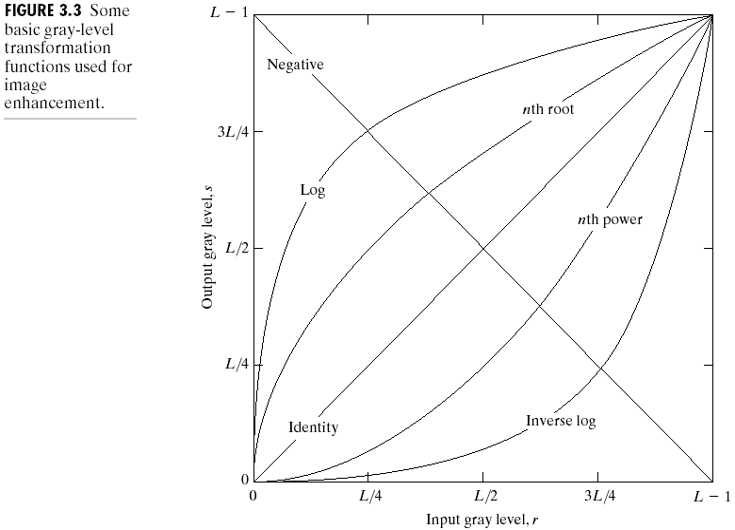
\includegraphics[width=0.6\linewidth]{fig/enhancement.png}
\end{figure}
\item 图像反转变换:$s=L-1-r$,人眼的一个特点就是在背景相对光亮时对灰度层次有较好的分辨能力。
\begin{figure}[H]
\centering
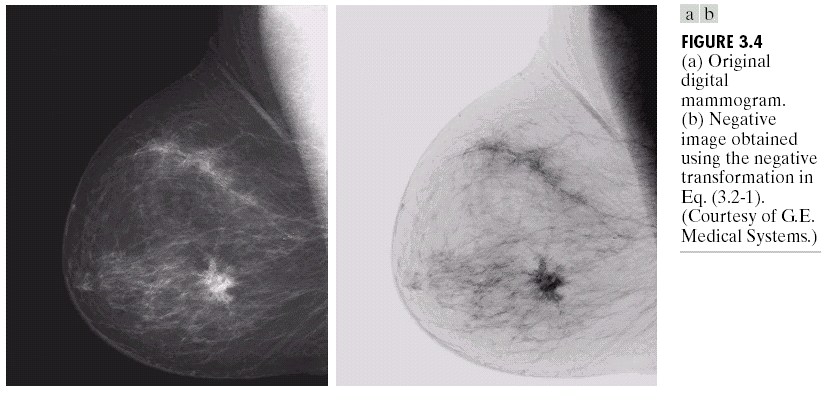
\includegraphics[width=0.6\linewidth]{fig/trans-inverse.png}
\end{figure}
\item 对数变换:$s=c\log(1+r)$,$c$是常数,$r\geq 0$,适合大范围的数据压缩。
任何具有对数函数曲线形状的变换都可以完成灰度的压缩和扩展功能。 
\begin{figure}[H]
\centering
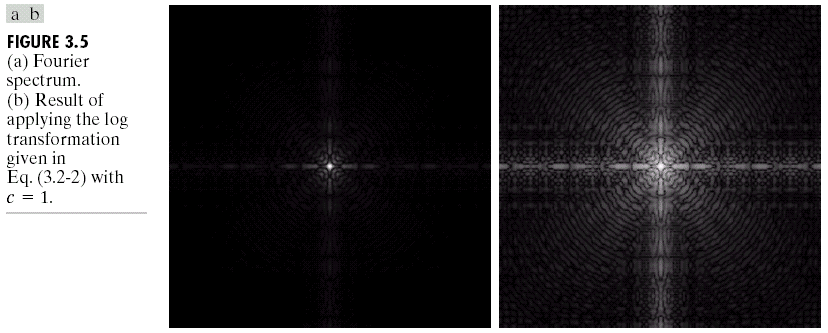
\includegraphics[width=0.6\linewidth]{fig/trans-log.png}
\end{figure}
\item 幂次变换:$s=cr^\gamma$,$c$和$\gamma$都为正常数
\begin{figure}[H]
\centering
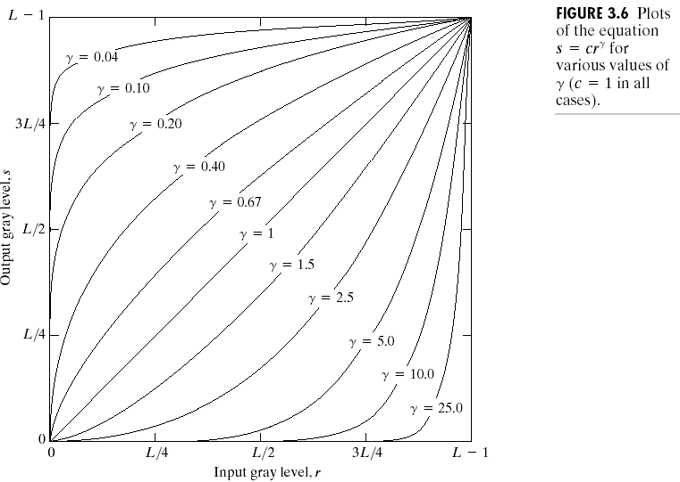
\includegraphics[width=0.6\linewidth]{fig/trans-power.png}
\end{figure}
伽马校正:大量的图像设备如捕捉卡、打印机、数码相机以及显示装置的响应(输出)就对应一个幂函数,通常称这个幂函数的指数为gamma。纠正这个幂次响应的处理称为伽玛校正(gamma correction)。
\begin{figure}[H]
\centering
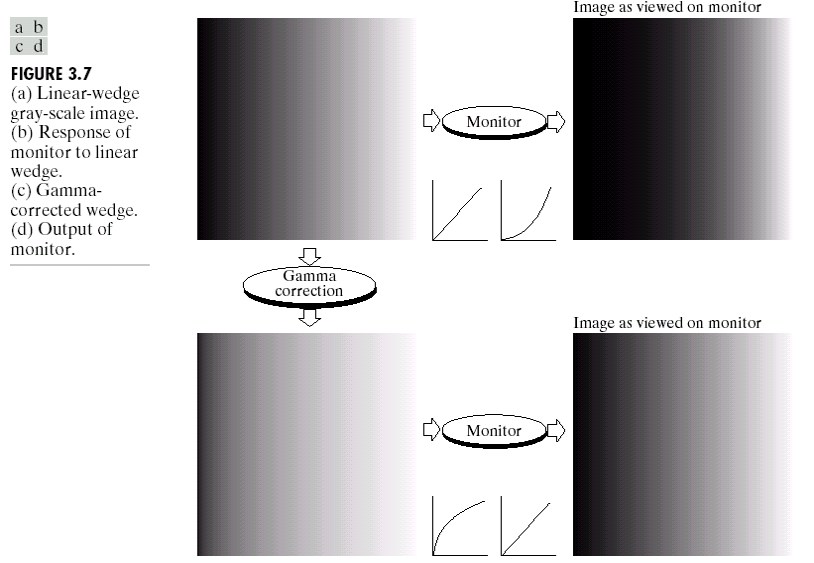
\includegraphics[width=0.6\linewidth]{fig/trans-gamma.png}
\end{figure}
在一般的图像处理软件中,几乎都有伽玛校正的功能。这个功能可用于调整图像的对比度。如果图像偏暗,有些低灰度值的细节被掩盖时,可考虑用指数$\gamma<1$的伽玛校正(变亮);反之,$\gamma>1$的校正对那些被“漂白”的细节会起作用(变暗)。
\item 分段线性变换
\begin{figure}[H]
\centering
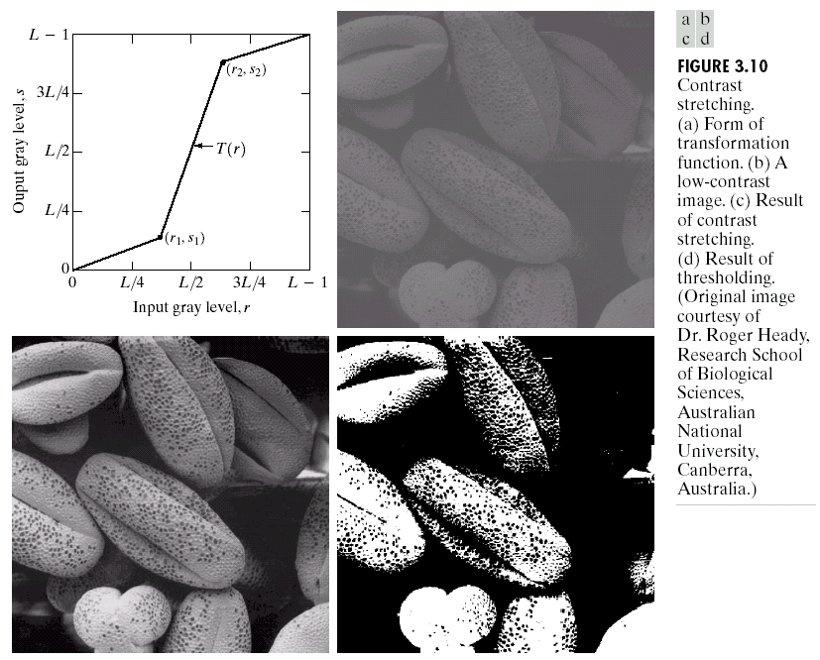
\includegraphics[width=0.6\linewidth]{fig/trans-by-cases.png}
\end{figure}
\item 灰度切割:在图像中提高特定灰度的亮度
\begin{figure}[H]
\centering
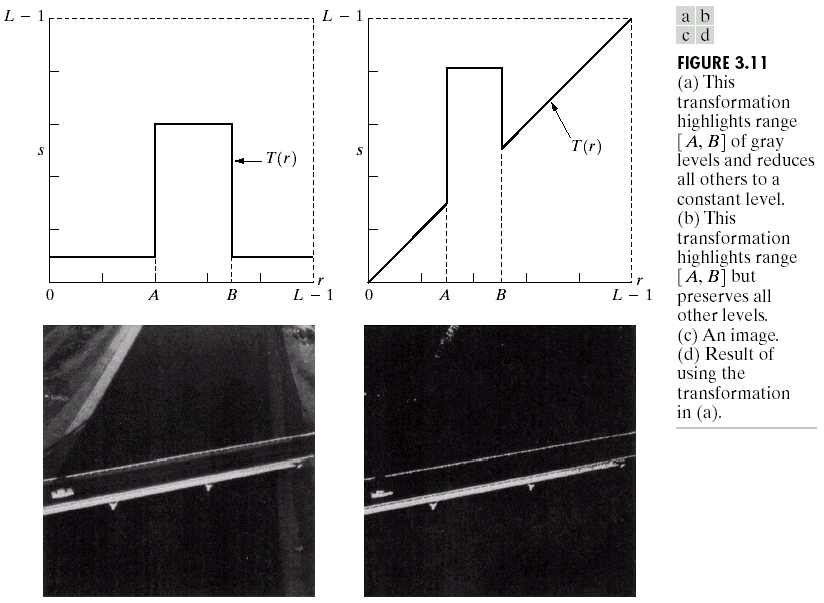
\includegraphics[width=0.6\linewidth]{fig/trans-cut.png}
\end{figure}
\end{itemize}

位图切割:8位灰度图象可以分割成8个位面,每个是一个二值图像(中间切一半)。
\textbf{高位}表示了\textbf{重要的信息},\textbf{低位}给出了\textbf{不同程度的细节}。
\begin{figure}[H]
\centering
\begin{tabular}{cc}
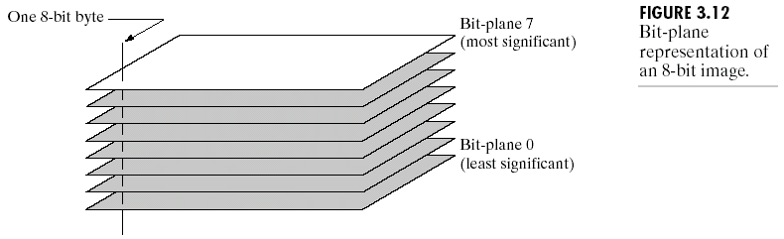
\includegraphics[width=0.5\linewidth]{fig/bitmap.png}&
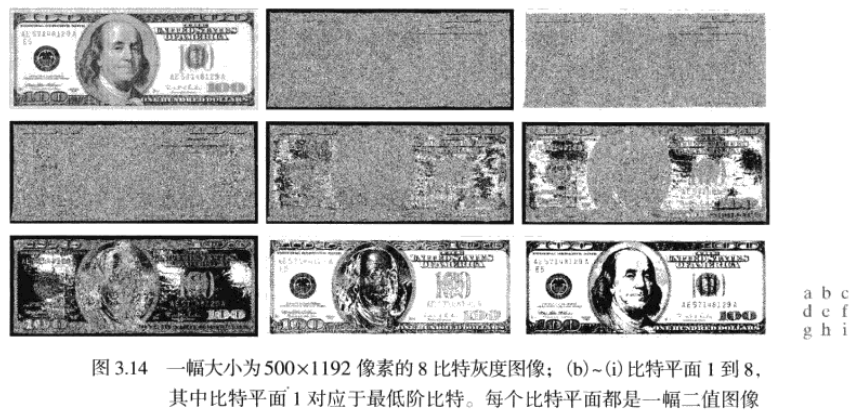
\includegraphics[width=0.5\linewidth]{fig/bitmap-dollars.png}
\end{tabular}
\end{figure}

位图的作用
\begin{itemize}
	\item 信息隐藏:藏在中间位,低位会被丢弃,高位太清楚
	\item 视频传输:先传高位,再传低位,逐渐清晰
\end{itemize}

\subsection{直方图}
\begin{definition}[直方图]
灰度级别为$[0,L-1]$(直方图一定从0开始!)。数字图像直方图是离散函数$h(r_k)=n_k$,其中$r_k$是第$k$级灰度,$n_k$是图像中灰度级为$r_k$的像素个数(频数)。
除以总数$n$就得到归一化的直方图。
\end{definition}

\subsubsection{直方图均衡化}
有亮度差才能看到细节,最好是均衡分布,实现\textbf{高对比度}。
\begin{figure}[H]
\centering
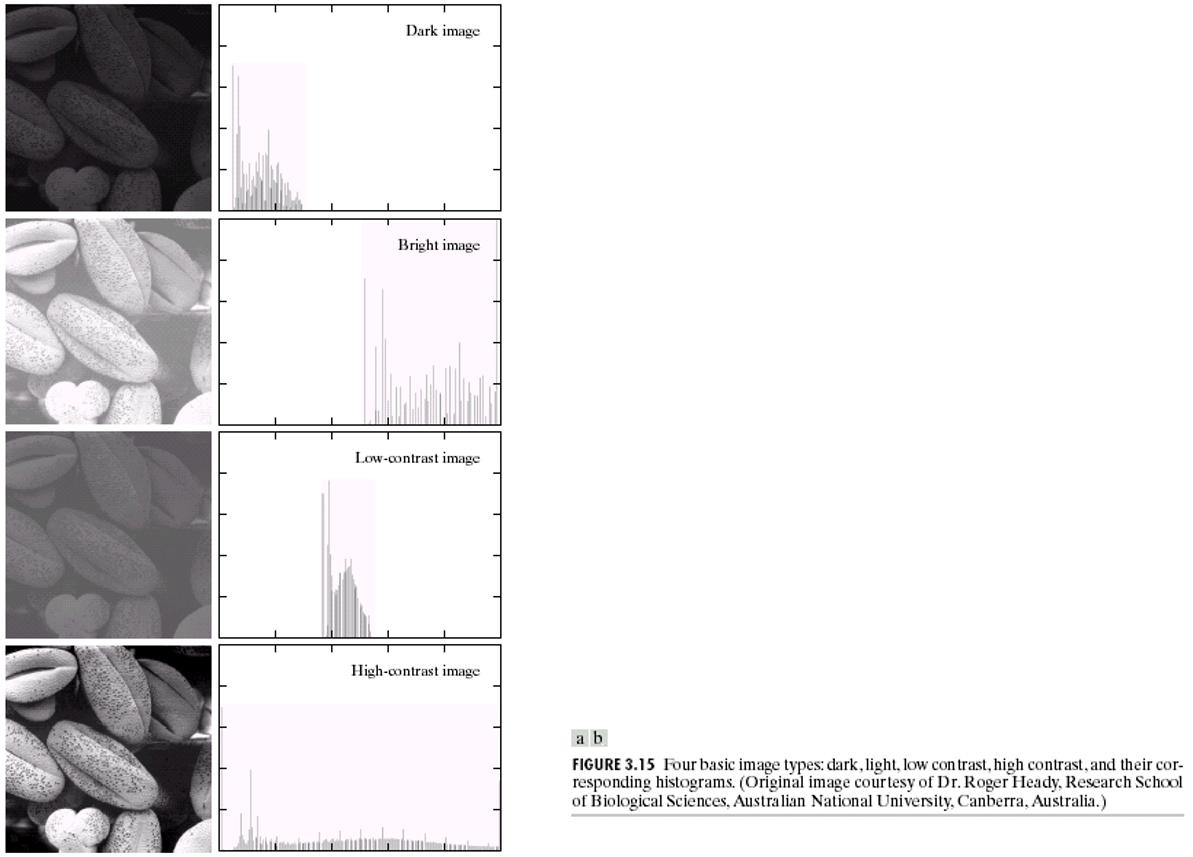
\includegraphics[width=0.6\linewidth]{fig/histogram-quality.png}
\end{figure}

直方图均衡化/线性化则是寻求一种变换使得变换后的图像具有尽可能均匀分布的直方图,用于图像增强最大的特点是自动化,有强大的适应性强的功能。
通常需要满足下列条件:
\begin{itemize}
	\item $T(r)$在$0\leq r\leq L-1$中为单值且单调递增
	\item 当$0\leq r\leq L-1$时,$0\leq T(r)\leq L-1$
\end{itemize}
步骤如下:
\begin{enumerate}
	\item 概率$p_r(r_k)=n_k/n,k=0,1,2,\ldots,L-1$
	\item 累计分布函数(PDF)
	\[P(r_k)=\sum_{j=0}^k p_r(r_j)=\sum_{j=0}^k\frac{n_j}{n},k=0,1,2,\ldots,L-1\]
	\item 变换函数
	\[s_k=T(r_k)=(L-1)\cdot\sum_{j=0}^k\frac{n_j}{n},k=0,1,2,\ldots,L-1\]
	\item 将$s_k$四舍五入转换为标准灰度级别,如有相同$\lceil s_k\rceil$则合并
\end{enumerate}
\begin{figure}[H]
\centering
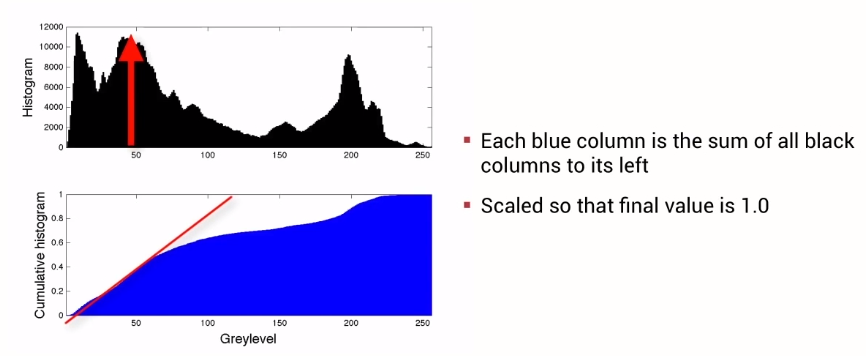
\includegraphics[width=0.8\linewidth]{fig/histogram-normalization.png}
\end{figure}
\begin{analysis}
若$r$为离散型随机变量,$T(r)$为单调递增函数($T^{-1}$存在且单调),且$s=T(r)$,则由概率论有
\[p_s(s)=p_r(r)\pd{r}{s}\Big|_{r=T^{-1}(s)}=p_s(T^{-1}(s))|T^{-1}(s)|\]
考虑变换函数为$r$的累积分布函数(CDF)
\[s=T(r)=\intabu{0}{r}{p_r(\omega)}{\omega}\]
对$s$求导并代入上面的式子可得$p_s(s)=1$,故实现均衡。
算法实际上就是求累积分布函数,使得原本亮度小的像素能够映射到亮度大的空间。
\end{analysis}

\subsubsection{直方图匹配}
当两幅图像比对时,通常要使其直方图形式一致(如不同光照条件下的同一场景)。
先是做空间归一化(伸缩、旋转),然后再做像素的归一化。

做法是使两幅图像均衡化后的结果相同,即
\[\begin{aligned}
s&=T(r)=\intabu{0}{r}{p_r(w)}{w}\\
s&=G(z)=\intabu{0}{z}{p_z(t)}{t}\\
\implies z&=G^{-1}(s)=G^{-1}(T(r))
\end{aligned}\]

具体步骤如下:
\begin{enumerate}
	\item 计算出原图的直方图
	\[s_k=T(r_k)=(L-1)\sum_{j=0}^k\frac{n_j}{n}\]
	\item 给出输出图像期望的直方图$p_z(z)$,并令
	\[v_k=G(z_k)=(L-1)\sum_{i=0}^kp_z(z_i)=s_k\]
	\item 寻找区间$[0,L-1]$的最小整数$\hat{z}$,使得
	\[G(\hat{z})-s_k\geq 0\]
	即由$k$映射到$\hat{z}$
\end{enumerate}

\begin{definition}[$n$阶矩]
设$p_r(r_k)=n_k/n$,则$r$的第$n$阶中心矩为
\[\mu_r(r_k)=\sum_{i=0}^{L-1}(r_i-\bar{r})^np(r_k)\]
其中$\bar{r}=\sum_{i=1}^{L-1}r_ip(r_i)$为$r$的平均值。
特别地,当$n=2$时为方差。
\end{definition}


\subsection{空间滤波基础}
滤波的概念来自信号处理中的傅里叶变换,空间滤波指的是直接对图像像素进行处理的操作。
滤波器(filter)有时也叫掩模(mask)、核(kernel)、模板(template)或窗口(window)。

\subsubsection{线性滤波}
空间域线性滤波基本公式:
\[g(x,y)=\sum_{s=-a}^a\sum_{t=-b}^b w(s,t)f(x+s,y+t)\]
常见的情况是,$a=b$为奇数,如1、3、5。

\begin{definition}[相关与卷积]
一个$m\times n$的滤波器$w(x,y)$与$M\times N$图像$f(x,y)$的相关操作定义为
\[w(x,y)\circ f(x,y)=\sum_{s=-a}^a\sum_{t=-b}^b w(s,t)f(x+s,y+t)\]
一个$m\times n$的滤波器$w(x,y)$与$M\times N$图像$f(x,y)$的卷积定义为
\[w(x,y)*f(x,y)=\sum_{s=-a}^a\sum_{t=-b}^b w(s,t)f(x-s,y-t)\]
其中右侧等号表示将$f$旋转$180\degree$(或先沿$x$轴翻折,再沿$y$轴翻折)
\end{definition}
\begin{figure}[H]
\centering
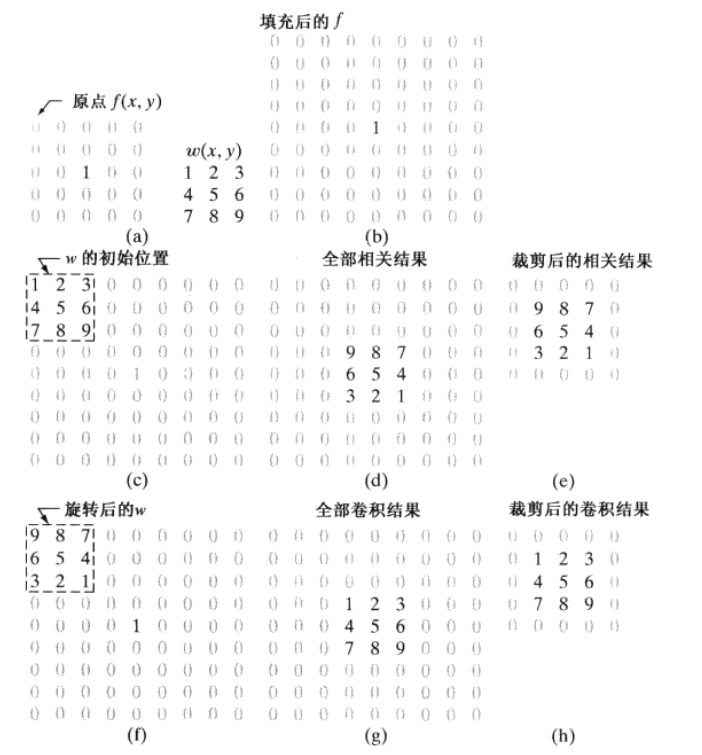
\includegraphics[width=0.5\linewidth]{fig/convolution_and_correlation.png}
\end{figure}

空间滤波对边界的处理方法
\begin{itemize}
	\item 重复边缘值
	\item 卷绕输入图像
	\item 补零(最常用)
	\item 勿略
\end{itemize}

常用的平滑滤波器(左侧是均值滤波)
\[g(x,y)=\frac{\disp\sum_{s=-a}^a\sum_{t=-b}^b w(s,t)f(x+s,y+t)}{\disp\sum_{s=-a}^a\sum_{t=-b}^b w(s,t)}\]
\begin{center}
\begin{tabular}{|c|c|c||c|c|c|}\hline
1/9 & 1/9 & 1/9 & 1/16 & 1/8 & 1/16\\\hline
1/9 & 1/9 & 1/9 & 1/8 & 1/4 & 1/8 \\\hline
1/9 & 1/9 & 1/9 & 1/16 & 1/8 & 1/16\\\hline
\end{tabular}
\end{center}

\subsubsection{非线性滤波}
排序统计滤波器是一种非线性的、 非卷积滤波器。
排序统计滤波器在滤波器包围的像素范围内排序,然后由统计排序结果决定的值代替中心像素的值。
按排序输出的位置分,可分为:中值滤波、最大值滤波、最小值滤波。

中值滤波比均值滤波更适合做\textbf{椒盐噪声}\footnote{特别大或特别小的噪声}的去除,因为噪声总是最大最小,故做中值滤波容易去除。
\begin{figure}[H]
\centering
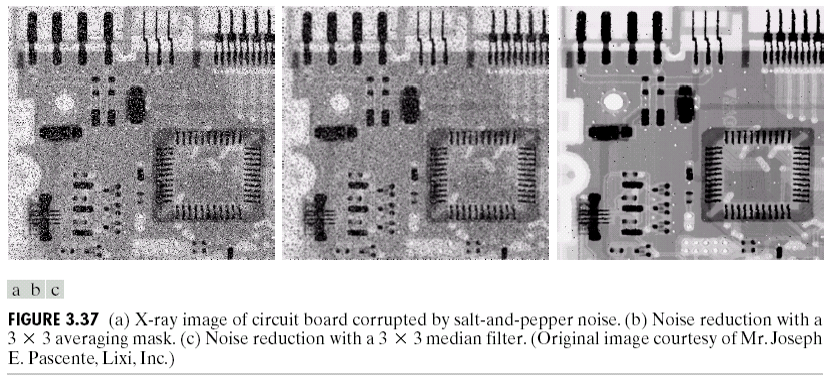
\includegraphics[width=0.8\linewidth]{fig/salt-and-pepper-noise.png}
\end{figure}

同理除了中值滤波,也可以构造第$X$百分点的滤波器。
通常$X<50$图像趋于变暗,$X>50$图像趋于变亮。


\subsection{图像锐化}
\subsubsection{图像微分}
\textbf{积分运算可以做平滑,微分运算可以做锐化!}
锐化的目的即突出图像中的细节或者增强被模糊的细节。

考虑离散情况
\[\begin{cases}
\pd{f}{x}&=f(x+1)-f(x)\\
\pdd{f}{x}&=f(x+1)+f(x-1)-2f(x)
\end{cases}\]

斜边缘、$\delta$/冲击边缘、阶梯边缘
\begin{figure}[H]
\centering
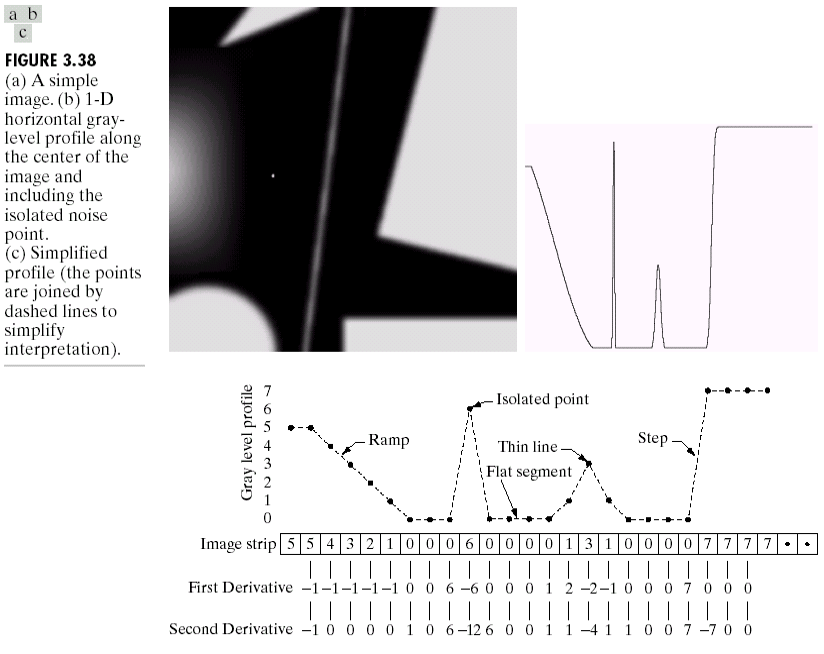
\includegraphics[width=0.6\linewidth]{fig/differential.png}
\end{figure}
\begin{itemize}
\item 一阶微分产生较“宽”的边界,二阶微分产生较“细”的边界
\item 二阶微分处理对细节有较强的响应,如细线和孤立点
\item 一阶微分对阶梯状的灰度变化有较强的响应
\item 二阶微分在处理阶梯状灰度变化时产生双响应
\item 如果灰度的变化相似,二阶微分对线的反应比对阶梯强,对点的反应比对线强
\end{itemize}

\subsubsection{拉普拉斯算子}
\begin{definition}[拉普拉斯(Laplacian)算子]
对连续函数情形,最简单且各向同性的二阶微分算子是拉普拉斯算子
\[\nabla^2 f=\pdd{f}{x}+\pdd{f}{y}\]
离散情况
\[\nabla^2=f(x+1,y)+f(x-1,y)+f(x,y+1)+f(x,y-1)-4f(x,y)\]
\end{definition}
拉普拉斯变换目的是\textbf{获得细节},加回原图像才能进行锐化。
\begin{figure}[H]
\centering
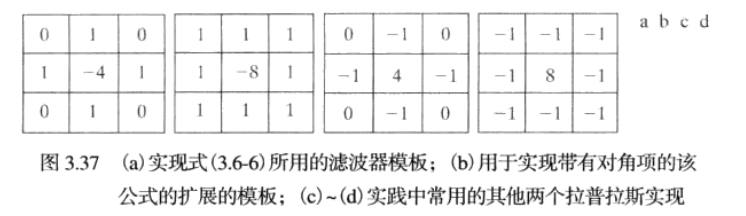
\includegraphics[width=0.6\linewidth]{fig/laplacian_mask.png}
\end{figure}

其实直接从滤波器的表示也可以直观看出这种滤波对图像的突变有比较强的响应(即在突变的位置有较大的输出值),对灰度变化缓慢的区域滤波响应的值会变得很小(变暗)。因此,用拉普拉斯算子作用后,产生的图像将是在暗背景上的一些灰色边线和一些突变点。若将原始图像叠加到拉普拉斯变换后的图像,既可以保护拉普拉斯锐化处理的效果,同时又能复原背景信息。 
拉普拉斯图像增强基本方法:
\[g(x,y)=\begin{cases}
f(x,y)-\nabla^2f & \text{拉普拉斯滤波中心系数为负}\\
f(x,y)+\nabla^2f & \text{拉普拉斯滤波中心系数为正}
\end{cases}\]
\begin{figure}[H]
\centering
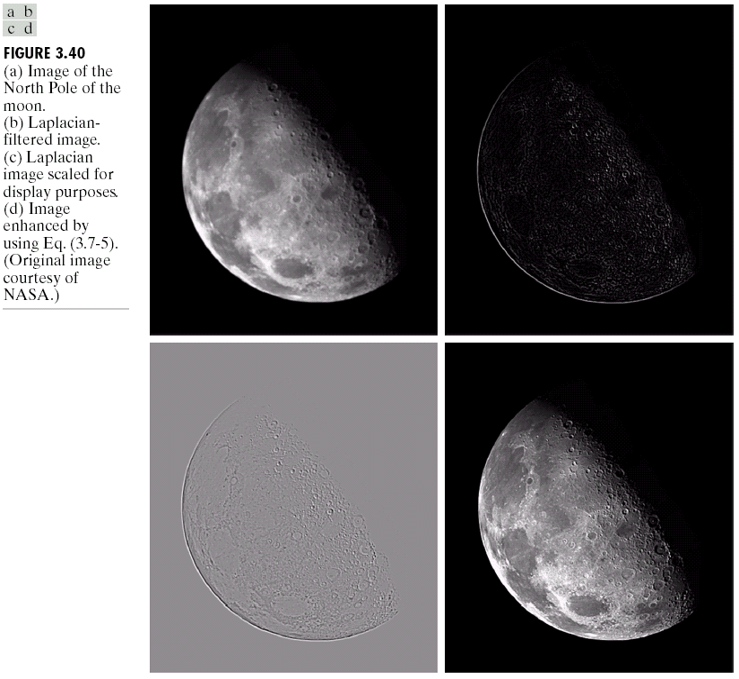
\includegraphics[width=0.6\linewidth]{fig/Laplacian.png}
\end{figure}

\begin{definition}[反锐化掩膜(unsharp masking)]
把原图的一个模糊过的图像从原图中减去,从而得到一个相对清晰的图像
\[f_s(x,y)=f(x,y)-\bar{f}(x,y)\]
就像一个模糊的负片和一个正片放在一起冲洗出相对清晰的照片
\end{definition}
\begin{definition}[高提升滤波(high-boost filtering)]
添加一个系数项$A$得到
\[f_{hb}(x,y)=Af(x,y)-\bar{f}(x,y)=(A-1)f(x,y)+f_s(x,y)\]
其中$A\geq 1$,目的为提升原图亮度,前一部分调整了原图的灰度,后一部分是锐化过的图像。
$A$越大则细节越不清晰,因为原图变亮了。
\end{definition}

可以得到基于拉普拉斯算子的高提升滤波
\[f_{hb}(x,y)=
\begin{cases}
Af(x,y)-\nabla^2 f & \text{Laplacian中心系数为负}\\
Af(x,y)+\nabla^2 f & \text{Laplacian中心系数为正}
\end{cases}\]
当$A=1$时就是拉普拉斯图像增强方法,当$A$足够大时,锐化效果将变得不明显。
\begin{figure}[H]
\centering
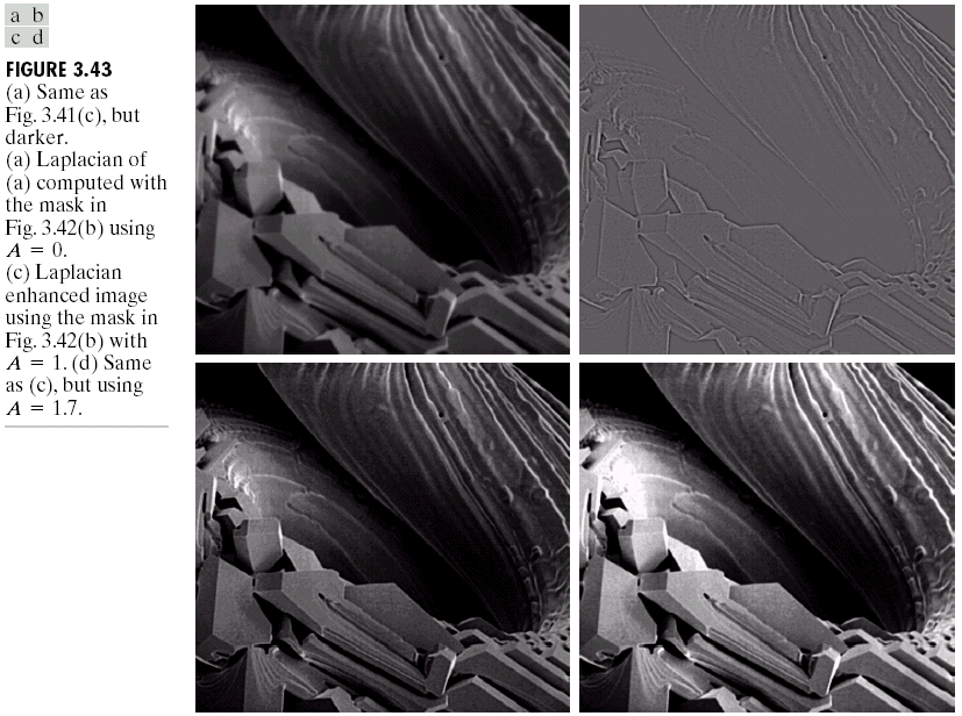
\includegraphics[width=0.6\linewidth]{fig/high-boost.png}
\end{figure}

\subsubsection{梯度}
一阶微分在灰度的跳跃性间断处(边界处)有较强的响应,所以在一些情况下也可以用于图像增强,常用作\textbf{边缘检测}。
考虑二维函数的梯度
\[\nabla\vf=\bmat{G_x & G_y}=\bmat{\pd{f}{x} & \pd{f}{y}}\]
定义$L_2$范数/模
\[\nabla f=(G_x^2+G_y^2)^{1/2}=\lrp{\lrp{\pd{f}{x}}^2+\lrp{\pd{f}{x}}^2}^{1/2}\]
$L_2$模具有各向同性的性质,但计算不方便,故常用$L_1$范数做代替
\[\nabla f\approx |G_x|+|G_y|\]
注意:通常在不引起混淆的情况下,把梯度的模称为梯度。
\begin{itemize}
\item Robert交叉梯度算子
\[\nabla f=|z_9-z_5|+|z_8-z_6|\]
\item Sobel算子:水平边缘增强
\[\nabla f=|(z_7+2z_8+z_9)-(z_1+2z_2+z_3)|+|(z_3+2z_6+z_9)-(z_1+2z_4+z_7)|\]
\begin{figure}[H]
\centering
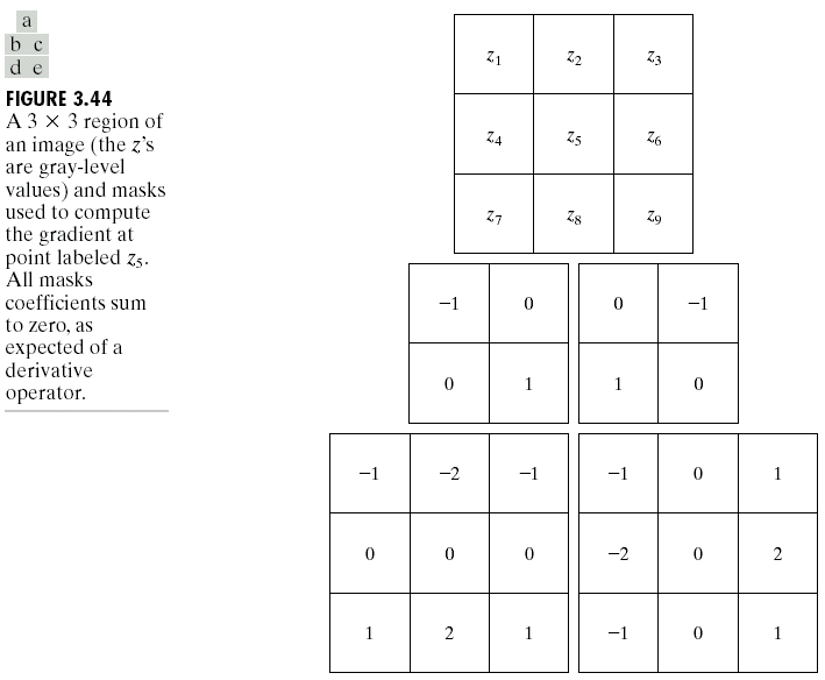
\includegraphics[width=0.4\linewidth]{fig/sobel_and_robert.png}
\end{figure}
\end{itemize}

通常实际使用时是多种滤波器混合使用。
下列为Matlab中预定义的滤波器。
\begin{itemize}
\item Gaussian 低通滤波器
\item Sobel 水平边缘增强滤波器
\item Prewitt 水平边缘增强滤波器:将Sobel的系数绝对值全改为1
\item Laplacian 近似二维拉普拉斯运算滤波器
\item Log (Laplacian of Gaussian)高斯拉普拉斯滤波器
\item Average 均值滤波器
\item Unsharp 模糊对比增强滤波器
\end{itemize}
% !TEX root = main.tex

\section{频率域滤波}
\subsection{傅里叶级数与傅里叶变换}
\begin{definition}[傅里叶级数]
设$f(t)$为以$T$为周期的函数,绝对可积,则$f(t)$可表示为
\[f(t)=\sum_{n=-\infty}^{\infty}c_n\ee^{j\frac{2\pi n}{T}t}\]
其中$j$为虚数单位,
\[c_n=\frac{1}{T}\intabu{-T/2}{T/2}{f(t)\ee^{-j\frac{2\pi n}{T}t}}{t},\,n=0,\pm 1,\pm 2,\ldots\]
\end{definition}

傅里叶级数中每一个基函数都是一个单频谐波,对应的系数/频谱表明原函数对这种频率成分贡献的大小(原函数在这个谐波上的投影)

\begin{definition}[冲激/狄利克$\delta$函数]
面积为1的长方形不断压扁,最后变成宽为0,高为无穷大的函数(左侧为连续情况,右侧为离散情况)
\[\delta(t)=\begin{cases}
\infty & t=0\\
0 & t\ne 0
\end{cases}\qquad
\delta(x)=\begin{cases}
1 & x=0\\
0 & x\ne 0
\end{cases}\]
即
\[\intab{-\infty}{\infty}{\delta(t)}=1
\qquad
\sum_{x=-\infty}^{\infty}\delta(x)=1\]
具有取样(sifting)特性
\[\intab{-\infty}{\infty}{f(t)\delta(t-t_0)}=f(t_0)
\qquad
\sum_{x=-\infty}^{\infty}f(x)\delta(x-x_0)=f(x_0)\]
\end{definition}
\begin{definition}[冲激串]
无限多个分离的周期冲激单元$\Delta T$之和
\[s_{\Delta T}(t)=\sum_{n=-\infty}^{\infty}\delta(t-n\Delta T)\]
\end{definition}
\begin{figure}[H]
\centering
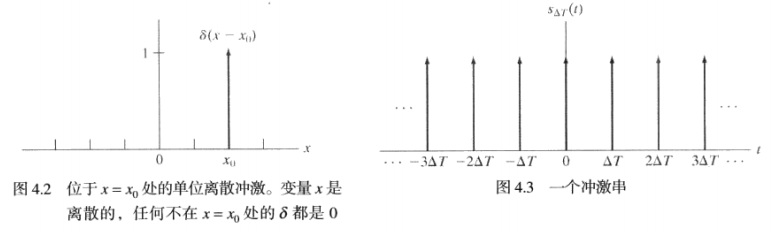
\includegraphics[width=0.8\linewidth]{fig/impulse.png}
\end{figure}

\begin{definition}[傅里叶变换与反变换]
连续情形的傅里叶变换(函数投影,取负号得共轭)和反变换为
\[\begin{aligned}
F(u)&=\Im[f(t)]=\intabu{-\infty}{+\infty}{f(t)\ee^{-j 2\pi ut}}{t}\\
f(t)&=\Im^{-1}[F(u)]=\intabu{-\infty}{+\infty}{F(u)\ee^{j 2\pi ut}}{u}
\end{aligned}\]
这两者构成一个傅里叶变换对。
对于离散情形有
\[\begin{aligned}
F(u)&=\sum_{x=0}^{M-1}f(x)\ee^{-j2\pi ux/M}\\
f(x)&=\frac{1}{M}\sum_{u=0}^{M-1}F(u)\ee^{j2\pi ux/M}
\end{aligned}\]
\end{definition}
由于傅里叶变换是$f(t)$乘上正弦项的展开,正弦项的频率由$\mu$决定(变量$t$已经被积分),积分后只剩下频率,故称傅里叶变换域是频率域。
注意坐标轴已经变化了,现在\textbf{横轴为频率}。

\begin{example}
矩形函数
\[f(t)=\begin{cases}
A & -W/2\leq t\leq W/2\\
0 & \text{otherwise}
\end{cases}\]
的傅里叶变换为
\[\begin{aligned}
F(u)&=\intabu{-W/2}{W/2}{A\ee^{-j2\pi ut}}{t}\\
&=\frac{-A}{j2\pi\mu}[\ee^{-j2\pi\mu W}-\ee^{j2\pi\mu W}]\\
&=AW\frac{\sin(\pi\mu W)}{\pi\mu W}=AW\sinc(\mu W)
\end{aligned}\]
\end{example}
\begin{example}
冲激的傅里叶变换(由取样特性)
\[F(\mu)=\intabu{-\infty}{\infty}{\delta(t)\ee^{-j2\pi\mu t}}{t}=\ee^{-j2\pi\mu 0}=1\]
而位于$t=t_0$的冲激傅里叶变换为
\[F(\mu)=\intabu{-\infty}{\infty}{\delta(t-t_0)\ee^{-j2\pi\mu t}}{t}=\ee^{-j2\pi\mu t_0}\]
周期冲激串的傅里叶变换
\[S(\mu)=\Im[s_{\Delta T}(t)]=\frac{1}{\Delta T}\sum_{n=-\infty}^{\infty}\delta\lrp{\mu-\frac{n}{\Delta T}}\]
\end{example}

\begin{definition}[卷积]
连续情形有
\[f(t)*h(t)=\intabu{-\infty}{+\infty}{f(\tau)h(t-\tau)}{\tau}\]
离散情形有
\[f(x)*h(x)=\sum_{m=0}^{M-1}f(m)h(x-m)\]
\end{definition}
\begin{theorem}[卷积定理]
建立起空间域和频率域\footnote{$t$所在的域称为空间域,$\mu$所在的域称为频率域}的联系
\[f(t)*h(t)\iff F(\mu)H(\mu)
\qquad
f(t)h(t)\iff F(\mu)*H(\mu)\]
即空间域两个函数卷积的傅里叶变换等于两个函数的傅里叶变换在频率域的乘积
\end{theorem}
\begin{analysis}
\[\begin{aligned}
\Im[f(t)*h(t)]&=\intabu{-\infty}{\infty}{\lrs{\intabu{-\infty}{\infty}{f(\tau)h(t-\tau)}{\tau}}\ee^{-j2\pi\mu t}}{t}\\
&=\intabu{-\infty}{\infty}{f(\tau)\lrs{\intabu{-\infty}{\infty}{h(t-\tau)\ee^{-j2\pi\mu t}}{t}}}{\tau}\\
&=\intabu{-\infty}{\infty}{f(\tau)\lrs{H(\mu)\ee^{-j2\pi\mu\tau}}}{\tau}\\
&=H(\mu)\intabu{-\infty}{\infty}{f(\tau)\lrs{\ee^{-j2\pi\mu\tau}}}{\tau}\\
&=H(\mu)F(\mu)
\end{aligned}\]
\end{analysis}

\subsection{取样函数}
\begin{example}
求取样函数
\[\tilde{f}(t)=f(t)s_{\Delta T}(t)=\sum_{n=-\infty}^{\infty}f(t)\delta(t-n\Delta T)\]
的傅里叶变换
\end{example}
\begin{analysis}
由卷积定理
\[\begin{aligned}
\tilde{F}(u)&=\Im[\tilde{f}(t)]=\Im[f(t)s_{\Delta T}(t)]\\
&=F(u)*S(u)=\intabu{-\infty}{\infty}{F(\tau)S(u-\tau)}{\tau}\\
&=\frac{1}{\Delta T}\intabu{-\infty}{\infty}{F(\tau)\sum_{n=-\infty}^{\infty}\delta\lrp{u-\tau-\frac{n}{\Delta T}}}{\tau}\\
&=\frac{1}{\Delta T}\sum_{n=-\infty}^{\infty}F\lrp{u-\frac{n}{\Delta T}}
\end{aligned}\]
\end{analysis}

\begin{theorem}[奈奎斯特(Nyquist)采样定理]
如果以超过函数最高频率的两倍的采样率来获得样本,则连续的带限函数\footnote{对于以原点为中心的有限区间(带宽)之外的频率值,其傅里叶变换为零。
}可以完全从它的样本集恢复,即
\[\frac{1}{\Delta T}>2\mu_{\max}\]
\end{theorem}

若以低于两倍的采样率来采样则会出现混淆现象
\begin{figure}[H]
\centering
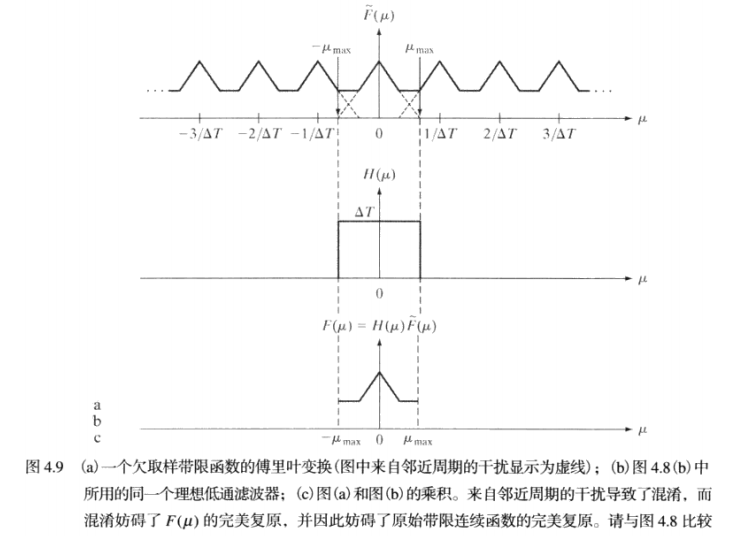
\includegraphics[width=0.8\linewidth]{fig/nyquist.png}
\end{figure}

由取样数据重建函数
\[f(t)=\sum_{n=-\infty}^{\infty}f(n\Delta T)\sinc\lrs{\frac{t-n\Delta T}{\Delta T}}\]

\subsection{二维傅里叶变换}
\begin{definition}[二维冲激]
\[\delta(t,z)=\begin{cases}
\infty & t=z=0\\
0 & \text{otherwise}
\end{cases}\qquad
\delta(x,y)=\begin{cases}
1 & x=y=0\\
0 & \text{otherwise}
\end{cases}\]
有取样特性
\[\sum_{x=-\infty}^\infty\sum_{y=-\infty}^\infty f(x,y)\delta(x-x_0,y-y_0)=f(x_0,y_0)\]
\end{definition}
\begin{definition}[二维离散傅里叶变换]
二维连续傅里叶变换对
\[\begin{aligned}
F(u,v)&=\intabu{-\infty}{\infty}{\intabu{-\infty}{\infty}{f(t,z)\ee^{-j2\pi(ut+vz)}}{t}}{z}\\
f(t,z)&=\intabu{-\infty}{\infty}{\intabu{-\infty}{\infty}{F(u,v)\ee^{j2\pi(ut+vz)}}{u}}{v}
\end{aligned}\]
二维离散傅里叶变换对
\[\begin{aligned}
F(u,v)&=\sum_{x=0}^{M-1}\sum_{y=0}^{N-1}f(x,y)\ee^{-2j\pi (ux/M+vy/N)}\\
f(x,y)&=\frac{1}{MN}\sum_{u=0}^{M-1}\sum_{v=0}^{N-1}F(u,v)\ee^{2\pi j(ux/M+vy/N)}
\end{aligned}\]
\end{definition}
\begin{theorem}[二维采样定理]
二维取样基于二维冲激串
\[\tilde{f}(t,z)=f(t,z)s_{\Delta T\Delta Z}(t,z)=\sum_{m=-\infty}^{\infty}\sum_{n=-\infty}^{\infty}f(t,z)\delta(t-m\Delta T,z-n\Delta Z)\]
取样率需要满足
\[\frac{1}{\Delta T}>2\mu_{\max}\qquad\frac{1}{\Delta Z}>2v_{\max}\]
\end{theorem}
\begin{definition}[傅里叶谱和相角]
由于二维DFT通常为复函数,因此用极坐标形式表示
\[F(u,v)=|F(u,v)|\ee^{j\varphi(u,v)}\]
其中幅度
\[|F(u,v)|=\sqrt{\Real^2(u,v)+\Imag^2(u,v)}\]
称为傅里叶谱,而
\[\varphi(u,v)=\arctan\lrs{\frac{\Imag(u,v)}{\Real(u,v)}}\]
为相角,
\[P(u,v)=|F(u,v)|^2\]
为功率谱
\end{definition}

注意$F(u,v)$的大小只是代表某一频率分量的数目,类似于直方图的概念。
频率域的坐标轴为$u,v$,因此中心点为$(0,0)$,
\[F(0,0)=\sum_{x=0}^{M-1}\sum_{y=0}^{N-1}f(x,y)=MN\bar{f}(x,y)\]
为图像的平均灰度。
即$u$方向和$v$方向上最低频的位置,零点处两个方向的频率都为零,因此这个量经常也被称为频谱的直流分量(DC)。

\begin{example}[陷波滤波器(notch filter)]
使得处理后的图像均值为0,从而使图像的整体灰度降低
\[H(u,v)=\begin{cases}
0 & (u,v)=(M/2,N/2)\\
1 & \text{others}
\end{cases}\]
\end{example}

\begin{figure}[H]
\centering
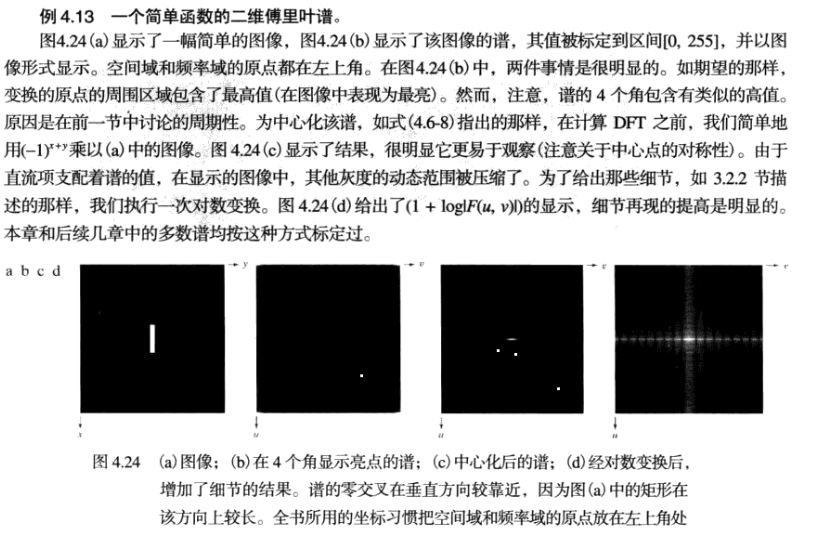
\includegraphics[width=\linewidth]{fig/fourier_spectrum.png}
\end{figure}

\textbf{相角对形状起着决定性作用!灰度信息则由谱携带。}
\begin{figure}[H]
\centering
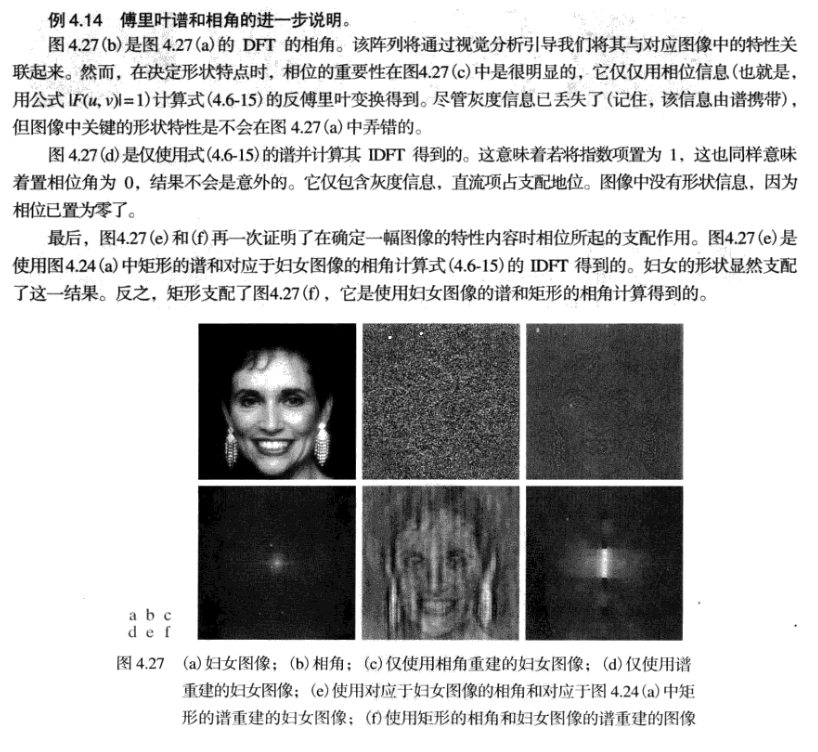
\includegraphics[width=\linewidth]{fig/spectrum_angle_example.png}
\end{figure}

\begin{theorem}[二维卷积定理]
二维的卷积定义如下
\[f(x,y)*h(x,y)=\sum_{m=0}^{M-1}\sum_{n=0}^{N-1}f(m,n)h(x-m,y-n)\]
同样有傅里叶变换对
\[\begin{aligned}
f(x,y)*h(x,y)\iff F(u,v)H(u,v)\\
f(x,y)h(x,y) \iff F(u,v)*H(u,v)
\end{aligned}\]
\end{theorem}
注意周期靠近会导致互相干扰而导致缠绕错误,因此需要进行零延拓(padding)。

假设函数$f(x)$和$h(x)$分别有$A$个和$B$个点组成,对这两个函数同时添加零,使其具有相同的周期
\[f_e=\begin{cases}
f(x) & 0\leq A-1\\
0 & A\leq x\leq P
\end{cases}
\qquad
h_e=\begin{cases}
h(x) & 0\leq x\leq B-1\\
0 & B\leq x\leq P
\end{cases}\]
同样对于二维图像滤波,若$f(x,y)$大小为$A\times B$,$h(x,y)$大小为$C\times D$,则延拓函数
\[f_e(x,y)=\begin{cases}
f(x,y) & 0\leq x\leq A-1\land 0\leq y\leq B-1\\
0 & A\leq x\leq P\lor B\leq y\leq Q
\end{cases}
\qquad
h_e(x,y)=\begin{cases}
h(x,y) & 0\leq x\leq C-1\land 0\leq y\leq D-1\\
0 & C\leq x\leq P\lor D\leq y\leq Q
\end{cases}\]
其中$P\geq A+C-1$,$Q\geq B+D-1$,通常可取$P=2M$,$Q=2N$。

\begin{definition}[相关]
相关性相当于算内积
\[g(x,y)=f(x,y)\circ h(x,y)=\sum_{m=0}^{M-1}\sum_{n=0}^{N-1}f^\star(m,n)h(x+m,y+n)\]
\end{definition}
\begin{theorem}[相关定理]
\[\begin{aligned}
f(x,y)\circ h(x,y)&\iff F^\star(u,v)H(u,v)\\
f^\star(x,y)h(x,y)&\iff F(u,v)\circ H(u,v)
\end{aligned}\]
\end{theorem}


\subsection{频率域滤波}
之所以要到频率域做滤波,是因为直观且计算比空间滤波容易(卷积耗时)
\begin{itemize}
\item 低通滤波器:平滑/模糊图像,设$D(u,v)$为频率域中点$(u,v)$与频率矩形中心的距离,$D_0$为截止频率
\begin{center}
\begin{tabular}{c|c|c}\hline
理想(ILPF) & $n$阶布特沃斯(BLPF) & 高斯\\\hline
$H(u,v)=\begin{cases}1 & D(u,v)\leq D_0\\0 & D(u,v)>D_0\end{cases}$ &
$H(u,v)=\dfrac{1}{1+[D(u,v)/D_0]^{2n}}$ &
$H(u,v)=\ee^{-D^2(u,v)/2D_0^2}$\\\hline
\end{tabular}
\end{center}
原点在频率中心,半径为$r$的圆包含的功率为
\[\alpha=\lrp{\sum_u\sum_v \frac{P(u,v)}{P_T}}\times 100\%=\lrp{\sum_u\sum_v \frac{P(u,v)}{\sum_{u=0}^{M-1}\sum_{v=0}^{N-1}|F(u,v)|^2}}\times 100\%\]
由于截止频率点处跳变太直接,物理无法实现,故是理想滤波器;而且会产生滤波模糊和振铃现象。
一阶BLPF没有振铃,二阶BLPF振铃很小,随着阶数增高振铃增大,故通常用二阶。
\item 高通滤波器:$H_{hp}(u,v)=1-H_{lp}(u,v)$,锐化图像(噪声、边缘、细节),只获得高频特征,没有背景,留下细节
\begin{center}
\begin{tabular}{c|c|c}\hline
理想(IGPF) & $n$阶布特沃斯(BGPF) & 高斯\\\hline
$H(u,v)=\begin{cases}0 & D(u,v)\leq D_0\\1 & D(u,v)>D_0\end{cases}$ &
$H(u,v)=\dfrac{1}{1+[D_0/D(u,v)]^{2n}}$ &
$H(u,v)=1-\ee^{-D^2(u,v)/2D_0^2}$\\\hline
\end{tabular}
\end{center}
\item 拉普拉斯滤波
\[H(u,v)=-4\pi^2\lrs{(u-P/2)^2+(v-Q/2)^2}=-4\pi^2D^2(u,v)\]
前面的系数可以去掉。拉普拉斯图像由下式给出
\[\nabla^2f(x,y)=\Im^{-1}[H(u,v)F(u,v)]\]
图像增强可以由下式实现
\[g(x,y)=f(x,y)+c\nabla^2 f(x,y)\]
\item 高频增强滤波:锐化/加强图像,高频增强,细节变得明显
\[\begin{aligned}
F_{lp}(u,v)&=H_{lp}(u,v)F(u,v)\\
F_{hp}(u,v)&=F(u,v)-F_{lp}(u,v)\\
&=(1-H_{lp}(u,v))F(u,v)\\
&=H_{hp}(u,v)F(u,v)\\
G(u,v)&=F(u,v)+F_{hp}(u,v)\\
&=(1+H_{hp}(u,v))F(u,v)
\end{aligned}\]
其中$k=1$为钝化模板,$k>1$为高提升滤波
\item 同态滤波器:高频增强,整个图像亮度又不能太亮(一片的亮度与低频有关)$\implies$抑制低频/环境光,提升高频/细节
\[f(x,y)=i(x,y)r(x,y)\]
其中$i(x,y)\in(0,\infty)$为照射分量(影响低频,一片);$0<r(x,y)<1$,反射率影响边缘/高频。
先取对数,然后再做傅里叶变换,最后记得取指数返回
\[\ln f(x,y)=\ln i(x,y)+\ln r(x,y)\]
同态滤波器
\[H(u,v)=(r_H-r_L)[1-\ee^{-c(D^2(u,v)/D_0^2)}]+r_L\]
其中$c$用于控制滤波器函数斜面的锐化,$r_L<1$,$r_H>1$
\begin{figure}[H]
\centering
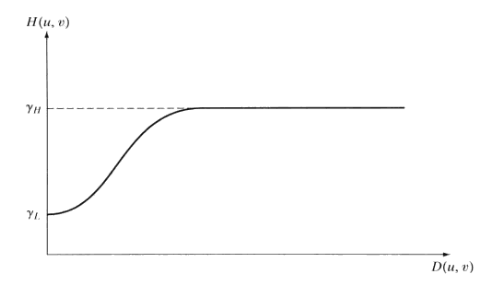
\includegraphics[width=0.4\linewidth]{fig/homo_filter.png}
\end{figure}
\end{itemize}

频率域滤波的步骤
\begin{figure}[H]
\centering
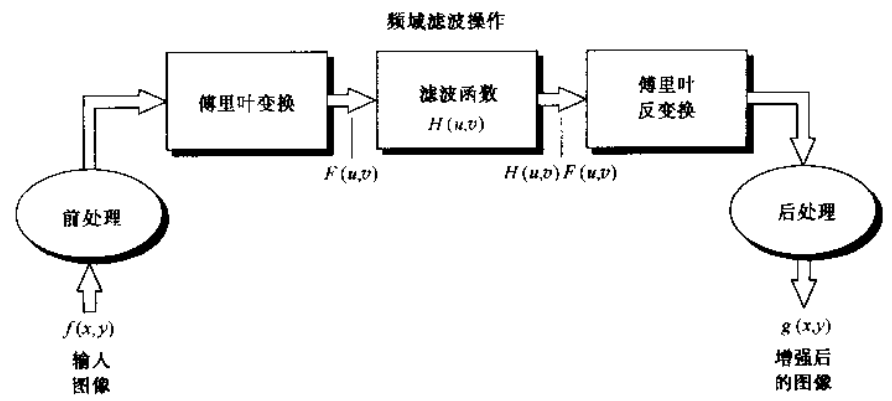
\includegraphics[width=0.6\linewidth]{fig/filter_pass.png}
\end{figure}
\begin{enumerate}
	\item 给定大小为$M\times N$的输入图像$f(x,y)$,选择填充参数$P=2M$,$Q=2N$
	\item 对$f(x,y)$添加必要的0,形成大小为$P\times Q$的填充后的图像$f_p(x,y)$
	\item 用$(-1)^{x+y}$乘以$f_p(x,y)$,做频谱中心化处理
	\item 用上面结果计算DFT,得到$F(u,v)$
	\item 生成一个\textbf{实对称}的滤波函数$H(u,v)$,大小为$P\times Q$,中心在$(P/2,Q/2)$处。
	用阵列相乘得到$G(u,v)=H(u,v)F(u,v)$
	\item 计算上式得到的IDFT,并恢复原图像
	\[g_p(x,y)=\Real[\Im[G(u,v)]](-1)^{x+y}\]
	\item 通过从$g_p(x,y)$的左上角提取$M\times N$大小的区域,得到最终结果$g(x,y)$
\end{enumerate}

\subsection{总结}
傅里叶变换的一些性质
\begin{itemize}
	\item 线性性:
	\[af_1(x,y)+bf_2(x,y)\iff aF_1(u,v)+bF_2(u,v)\]
	\item 平移性质:
	\[\begin{aligned}
	&f(x,y)\ee^{j2\pi(u_0x/M+v_0y/N)}\iff F(u-u_0,v-v_0)\\
	&f(x-x_0,y-y_0)\iff F(u,v)\ee^{-2j\pi(x_0u/M+y_0v/N)}
	\end{aligned}\]
	特别地,平移到频率矩形中心$(M/2,N/2)$
	\[\begin{aligned}
	&f(x,y)(-1)^{x+y}\iff F(u-M/2,v-N/2)\\
	&f(x-M/2,y-N/2)\iff F(u,v)(-1)^{u+v}
	\end{aligned}\]
	\item 旋转性质:使用极坐标$x=r\cos\theta,y=r\sin\theta,u=\omega\cos\varphi,v=\omega\sin\varphi$,有
	\[f(r,\theta+\theta_0)\iff F(\omega,\varphi+\varphi_0)\]
	\item 周期性:
	\[\begin{aligned}
	F(u,v)&=F(u+k_1M,v+k_2N)\\
	f(x,y)&=f(x+k_1M,y+k_2N)
	\end{aligned}\]
	\item 对称性:
	实函数$f(x,y)$的傅里叶变换是共轭对称/哈密特对称的
	\[F^\star(u,v)=F(-u,-v)\]
	而虚函数$f(x,y)$的傅里叶变换是共轭反对称的
	\[F^\star(-u,-v)=-F(u,v)\]
	\item 可分性:2D-FFT可变成两个1D-FFT
	\[F(u,v)=\sum_{x=0}^{M-1}\lrp{\sum_{y=0}^{N-1}f(x,y)\ee^{-j2\pi ux/M}}\ee^{-j2\pi vy/N}\]
\end{itemize}

常见函数的傅里叶变换
\begin{center}
\begin{tabular}{|c|l|}\hline
离散单位冲激 & $\delta(x,y)\iff 1,\;1\iff\delta(u,v)$\\\hline
矩形函数 & $\mathrm{rect}[a,b]\iff ab\frac{\sin(\pi ua)}{\pi ua}\frac{\sin(\pi ub)}{\pi ub}\ee^{-j\pi(ua+vb)}$\\\hline
正弦函数 & $\sin(2\pi u_0x+2\pi v_0y)\iff j\frac{1}{2}[\delta(u+Mu_0,v+Nv_0)-\delta(u-Mu_0,v-Nv_0)]$\\\hline
余弦函数 & $\cos(2\pi u_0x+2\pi v_0y)\iff j\frac{1}{2}[\delta(u+Mu_0,v+Nv_0)+\delta(u-Mu_0,v-Nv_0)]$\\\hline
微分 & $\frac{\diff^n f(x)}{\diff x^n}\iff (ju)^n F(u),\;\lrp{\pd{}{t}}^m\lrp{\pd{}{z}}^nf(t,z)\iff(j2\pi u)^m(j2\pi v)^nF(u,v)$\bigstrut\\\hline
高斯 & $A2\pi\sigma^2\ee^{-2\pi^2\sigma^2(t^2+z^2)}\iff A\ee^{-(u^2+v^2)/2\sigma^2}$\\\hline
\end{tabular}
\end{center}

用前向变换计算傅里叶反变换,以消除两套冗余电路
\[MNf^\star(x,y)=\sum_{u=0}^{M-1}\sum_{v=0}^{N-1} F^\star(u,v)\ee^{-j2\pi (ux/M+vy/N)}\]
% !TEX root = main.tex

\section{图像复原}
图像增强是主观的,图像复原则是客观的(恢复原图)。

空间域和频率域的退化图像分别可以由下式的退化模型给出
\[\begin{aligned}
g(x,y)&=h(x,y)*f(x,y)+\eta(x,y)\\
G(u,v)&=H(u,v)F(u,v)+N(u,v)
\end{aligned}\]
关键在于怎么找回$f$和$F$,而$h$属于系统噪声。

\begin{figure}[H]
\centering
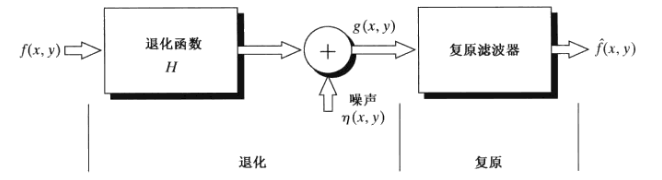
\includegraphics[width=0.8\linewidth]{fig/restoration.png}
\end{figure}

\subsection{噪声模型}
\begin{itemize}
\item 高斯噪声
\[p(z)=\frac{1}{\sqrt{2\pi}\sigma}\ee^{-\frac{(z-\bar{z})^2}{2\sigma^2}}\]
\item 脉冲/椒盐噪声
\[p(z)=\begin{cases}
P_a & z=a\\
P_b & z=b\\
1-P_a-P_b & \text{others}
\end{cases}\]
\item 瑞利噪声:均值$\bar{z}=a+\sqrt{\pi b/4}$,方差$\sigma^2=b(4-\pi)/4$
\[p(z)=\begin{cases}
\frac{2}{b}(z-a)\ee^{-(z-a)^2}{b} & z\geq a\\
0 & z<a
\end{cases}\]
\item 爱尔兰/伽马噪声:均值$\bar{z}=b/a$,方差$\sigma^2=b/a^2$
\[p(z)=\begin{cases}
\frac{a^bz^{b-1}}{(b-1)!}\ee^{-az} & z\geq a\\
0 & z<a
\end{cases},\;a>0,b\in\zz^+\]
\item 指数噪声:均值$\bar{z}=1/a$,方差$\sigma^2=1/a^2$
\[p(z)=\begin{cases}
a\ee^{-az} & z\geq 0\\
0 & z<0
\end{cases}\]
\item 均匀噪声:均值$\bar{z}=(a+b)/2$,方差$\sigma^2=(b-a)^2/12$
\[p(z)=\begin{cases}
\frac{1}{b-a} & a\leq z\leq b\\
0 & \text{others}
\end{cases}\]
\end{itemize}
\begin{figure}[H]
\centering
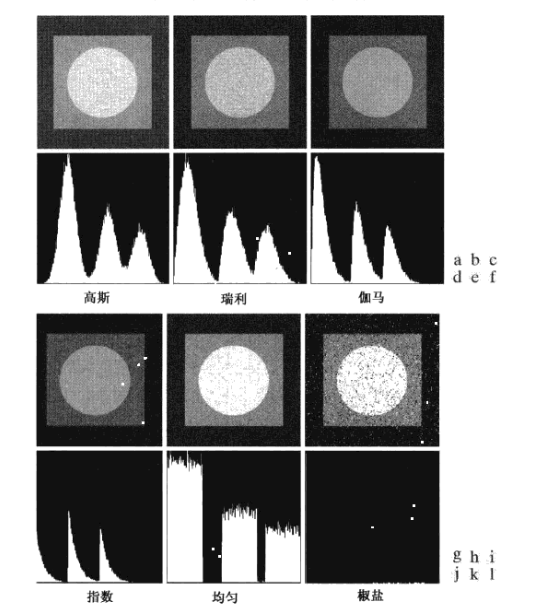
\includegraphics[width=0.5\linewidth]{fig/noise.png}
\end{figure}

\subsection{噪声存在下的空间滤波复原}
考虑唯一存在噪声退化,即不存在系统退化,则原式变为
\[\begin{aligned}
g(x,y)&=f(x,y)+\eta(x,y)\\
G(u,v)&=F(u,v)+N(u,v)
\end{aligned}\]

\subsubsection{均值滤波器}
\begin{itemize}
	\item 算术均值滤波
	\[\hat{f}(x,y)=\frac{1}{MN}\sum_{(s,t)\in S_{xy}}g(s,t)\]
	\item 几何均值滤波
	\[\hat{f}(x,y)=\lrs{\prod_{(s,t)\in S_{xy}}g(s,t)}^{\frac{1}{mn}}\]
	相比算术均值,丢失图像细节比较少
	\item 谐波均值滤波
	\[\hat{f}(x,y)=\frac{mn}{\sum_{(s,t)\in S_{xy}}\frac{1}{g(s,t)}}\]
	对盐(大的)噪声比较好,对胡椒噪声不好,善于处理高斯噪声
	\item 逆谐波均值滤波
	\[\hat{f}(x,y)=\frac{\sum_{(s,t)\in S_{xy}}g(s,t)^{Q+1}}{\sum_{(s,t)\in S_{xy}}g(s,t)^Q}\]
	其中$Q$称为滤波器的阶数,适合减少椒盐噪声的影响。
	当$Q$为正时,消除胡椒噪声;当$Q$为负时,消除盐粒噪声;但不能同时消除这两种噪声。
	当$Q=0$时退化为算术均值,$Q=-1$为谐波均值滤波
\end{itemize}

\subsubsection{状态/顺序统计滤波器}
\begin{itemize}
	\item 最大滤波器
	\item 最小滤波器
	\item \textbf{中点}滤波器:
	\[\hat{f}(x,y)=\frac{1}{2}[\max_{(x,y)\in S_{xy}}g(s,t)+\min_{(x,y)\in S_{xy}}g(s,t)]\]
	\item 修正阿尔法均值滤波器:去除$d/2$个最大值(去盐)和$d/2$最小值(去椒),再取平均(去高斯)
	\[\hat{f}(x,y)=\frac{1}{mn-d}\sum_{(x,y)\in S_{xy}}g_r(s,t)\]
\end{itemize}

\subsubsection{自适应滤波器}
滤波器作用于局部区域$S_{xy}$,$\sigma^2_\eta$为干扰$f(x,y)$以形成$g(x,y)$的噪声方差,$m_L$为局部均值,$\sigma_L^2$为局部方差
\[\hat{f}(x,y)=g(x,y)-\frac{\sigma^2_\eta}{\sigma^2_L}[g(x,y)-m_L]\]
满足以下假设
\begin{itemize}
	\item 如果$\sigma_\eta^2$为$0$,则应直接返回$g(x,y)$的值
	\item 如果局部方差与$\sigma_\eta^2$高度相关,则滤波器返回$g(x,y)$的近似值。
	典型地,高局部方差与边缘相关,应该保护这些边缘
	\item 如果两个方差相等,则希望滤波器返回$S_{xy}$中像素的算术均值。这种情况发生在局部区域与整个图像有相同特性地条件下,局部噪声将通过简单地求平均来降低。
\end{itemize}

\subsection{通过频域滤波抑制噪声}
\subsubsection{带阻滤波器}
只有中间$W$宽度的能够通过,同样有理想带阻滤波器、布特沃斯滤波器、高斯带阻滤波器
\[H(u,v)=\begin{cases}
1 & D(u,v)<D_0-\frac{W}{2}\lor D(u,v)>D_0+\frac{W}{2}\\
0 & \text{otherwise}
\end{cases}\]
带阻滤波可以消除周期性噪声。
\begin{figure}[H]
\centering
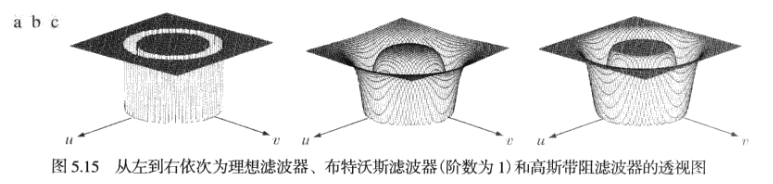
\includegraphics[width=0.8\linewidth]{fig/BSF.png}
\end{figure}

\subsubsection{带通滤波器}
\[H_{bp}(u,v)=1-H_{br}(u,v)\]
只是将带阻滤波器取反

\subsubsection{陷波滤波器}
阻止(或通过)事先定义得中心频率邻域内的频率
\begin{figure}[H]
\centering
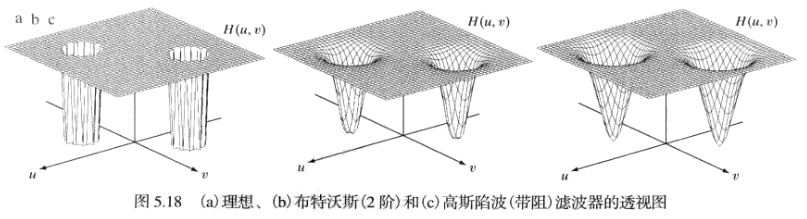
\includegraphics[width=0.8\linewidth]{fig/notch.png}
\end{figure}

由于频率域的共轭对称性,去掉一个,要去除另一个对称的频率。

陷波带通滤波器可以用于确定噪声模式。

如何评判图像的好坏
\begin{itemize}
\item 方差最小,噪声水平最低
\item 是不是平滑的
\end{itemize}

\subsection{线性、位置不变的退化}
输入/输出关系可以表示为
\[g(x,y)=H[f(x,y)]+\eta(x,y)\]

具有加性噪声的线性空间不变退化系统,可在空间域建模为退化(点扩散)函数与一幅图像的卷积,然后再加上噪声。
基于卷积定理,在频率域中,同样的过程可表示为图像和退化函数的变换的乘积,然后再加上噪声的变换。

\subsection{估计退化函数}
\begin{itemize}
	\item 观察法
	\[H_s(u,v)=\frac{G_s(u,v)}{\hat{F}_s(u,v)}\]
	\item 实验法:获取与退化图像类似的装置,由成像一个亮点得到退化的冲激响应
	\[A\delta(x,y)\to g(x,y)\iff A\to G(u,v)\]
	故$H(u,v)=\frac{G(u,v)}{A}$
	\item 数学建模法:如运动模糊
	\[g(x,y)=\intabu{0}{T}{f[x-x_0(t),y-y_0(t)]}{t}\]
	最终得到退化函数
	\[H(u,v)=\intabu{0}{T}{\ee^{-j2\pi[ux_0(t)+vy_0(t)]}}\]
\end{itemize}

\subsection{逆滤波}
对于线性移不变系统的退化模型为
\[G(u,v)=H(u,v)F(u,v)+N(u,v)\]
如果知道$H(u,v)$,则可以计算原始图像的傅里叶变换估计(去卷积)
\[\hat{F}(u,v)=\frac{G(u,v)}{H(u,v)}=F(u,v)+\frac{N(u,v)}{H(u,v)}\]
如果$H(u,v)$很小,则$N(u,v)/H(u,v)$将很大,估计就会失败。

维纳滤波:最佳去噪滤波器
\[\hat{F}(u,v)=\frac{P_f(u,v)}{P_f(u,v)+P_k(u,v)}=\frac{P_f(u,v)}{P_f(u,v)+\lrabs{\frac{N(u,v)}{H(u,v)}}}\]
% !TEX root = main.tex

\section{彩色图像处理}
图像主要包括三方面内容:颜色、形状、纹理

\subsection{颜色特性}
彩色光的3个基本量:
\begin{itemize}
	\item 辐射率:从光源流出能量的总量,用Watt表示
	\item 光强:观察者从光源接受的能量总和,用流明表示
	\item 亮度:主观描绘子,人感觉到的
\end{itemize}

人眼中有600-700万个锥状体分别对红色(700nm)、绿色(546nm)、蓝色(435.8nm)敏感\footnote{注意这里只是人为定义波长,真正的红绿蓝是一段波长区间。}。
65\%对红光敏感、33\%对绿光敏感、2\%对蓝光敏感。

三基色原理:
红绿蓝为三种基色,组成RGB三维加性空间
\begin{figure}[H]
\centering
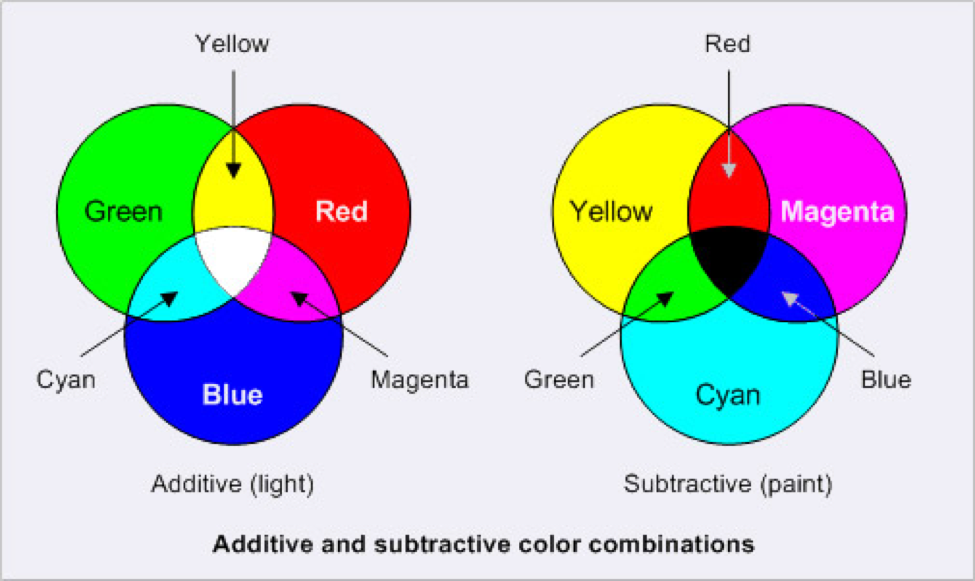
\includegraphics[width=0.8\linewidth]{fig/rgb_and_cmyk.png}
\end{figure}

区别颜色的特性:亮度、色调、色饱和度。
颜色通常用亮度和彩色表征,色调、和饱和度统称为彩色色度。
设$X,Y,Z$为红绿蓝的系数,则做归一化,得到颜色的唯一比例
\[\begin{aligned}
x&=\frac{X}{X+Y+Z}\\
x&+y+z=1
\end{aligned}\]

真彩色(24b):RGB各用一个字节表示,共216种安全色(各种设备都可以正常显示),剩下40个为控制字节

\subsection{颜色空间}
常见的颜色空间\footnote{\url{https://en.wikipedia.org/wiki/List_of_color_spaces_and_their_uses}}如下
\begin{itemize}
	\item RGB:\textbf{加性空间},与人眼视觉系统密切相连。
	\begin{itemize}
		\item RGBA:加上透明通道
		\item sRGB(standard):Microsoft
		\item Adobe RGB:打印出来更接近原色
	\end{itemize}
	\item CMY/CMYK:青色(cyan)、品红(magenta)、黄色(yellow)、黑色(key/black),主要用于\textbf{打印}。打印主要靠反射(\textbf{减性空间}),如黄色是白光将蓝色吸收掉。由于油墨很少能将颜色都吸收掉,深色效果较差,故加入一种黑色K。
	\item HIS/HSL/HSV:色度(hue)、亮度(intensity)、饱和度(saturation),亮度与色彩分离。广泛应用于计算机视觉、图像检索和视频检索。
	\item CIE:第一个基于人类视觉感知的颜色空间。CIE-XYZ(1931)是在RGB系统的基础上,用数学方法,选用三个理想的原色来代替实际的三原色,从而将CIE-RGB系统中的光谱三刺激值和色度坐标r、g、b均变为正值。
	\item Lab:Lab模式既不依赖光线,也不依赖于颜料,它是CIE组织确定的一个理论上包括了人眼可以看见的所有色彩的色彩模式。Lab模式弥补了RGB和CMYK两种色彩模式的不足。同RGB颜色空间相比,Lab是一种不常用的色彩空间。它是一种设备无关的颜色系统,也是一种基于生理特征的颜色系统。
	这也就意味着,它是用数字化的方法来描述人的视觉感应。Lab颜色空间中的L分量用于表示像素的亮度,取值范围是$[0,100]$,表示从纯黑到纯白;a表示从红色到绿色的范围,取值范围是$[127,-128]$;b表示从黄色到蓝色的范围,取值范围是$[127,-128]$。
	\item YUV:明亮度(Y, Luminance/Luma)即灰阶值、色度(U/V, Chrominance/Chroma)用于指定像素颜色。包括YCbCr、YPbPr、YUV、Y'UV等,后两者通常用来编码电视的模拟信号\footnote{Y'UV的发明是由于彩色电视与黑白电视的过渡时期。黑白视频只有Y(Luma/Luminance)视频,也就是灰阶值。到了彩色电视规格的制定,是以YUV/YIQ的格式来处理彩色电视图像,把UV视作表示彩度的C(Chrominance或Chroma),如果忽略C信号,那么剩下的Y(Luma)信号就跟之前的黑白电视频号相同,这样一来便解决彩色电视机与黑白电视机的兼容问题。Y'UV最大的优点在于只需占用极少的带宽。},YCbCr用来描述数字的视频信号,适合视频与图片压缩以及传输,例如MPEG、JPEG。
\end{itemize}

关于不同颜色空间的优缺点可见\footnote{\url{https://blog.csdn.net/JiangHui1211/article/details/84592774}}。

\subsection{伪彩色处理}
根据一定的准则对灰度值赋以彩色的处理。
之所以需要伪彩色,是因为人类可以辨别上千种颜色和强度,但只能辨别二十几种\textbf{灰度}。
比如将不同灰度赋予不同颜色,得到热度图(heatmap)。

\subsection{全彩色处理}
两种处理方式:分通道处理、向量处理。

补色:两种颜色混在一起为白色(RGB补色为CMY)
\begin{figure}[H]
\centering
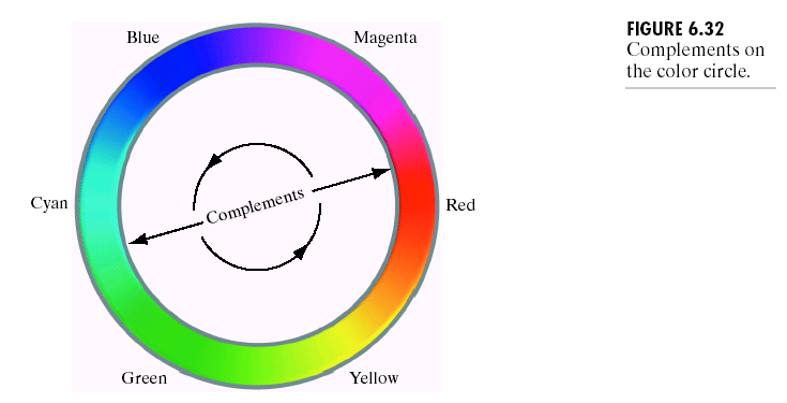
\includegraphics[width=0.6\linewidth]{fig/complements.png}
\end{figure}

\subsection{彩色分割}
\begin{itemize}
	\item HSI颜色空间分割直观,H色调图像方便描述彩色,S饱和度图像做模板分离感兴趣的特征区,I强度图像不携带彩色信息。如用门限产生二值图像,大于门限的像素赋为1,其他赋为0。
	\item RGB彩色空间直接,用欧式距离度量。
\end{itemize}
% 彩色空间的人脸检测

如果直接采用3个独立平面形成的合成梯度图可能导致彩色边缘检测错误,因此要采用Di Zenzo提出的方法。
% !TEX root = main.tex

\section{形态学图像处理}
\subsection{腐蚀与膨胀}
\begin{definition}[反射]
\[\hat{B}=\{w\mid w=-b,b\in B\}\]
\end{definition}
\begin{definition}[平移]
\[(B)_z=\{c\mid c=b+z,b\in B\}\]
\end{definition}
\begin{definition}[腐蚀]
结构元$B$可以完全含于$A$中
\[A\ominus B=\{z\mid(B)_z\subset A\}=\{z\mid(B)_z\cap A^C=\varnothing\}\]
注意最终结果只保留结构元的中心点。
腐蚀可以消除图像中的某些部分。
\end{definition}
\begin{figure}[H]
\centering
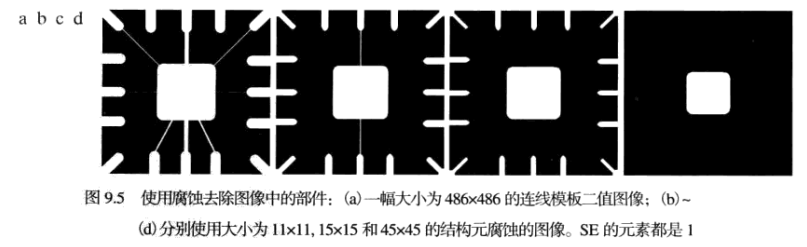
\includegraphics[width=0.9\linewidth]{fig/erosion.png}
\end{figure}
\begin{definition}[膨胀]
结构元$B$与$A$有交
\[A\oplus B=\{z\mid(\hat{B})_z\cup A\ne\varnothing\}=\{z\mid [(\hat{B})_z\cap A]\subset A\}\]
膨胀可以用来桥接裂缝。
\end{definition}
\begin{figure}[H]
\centering
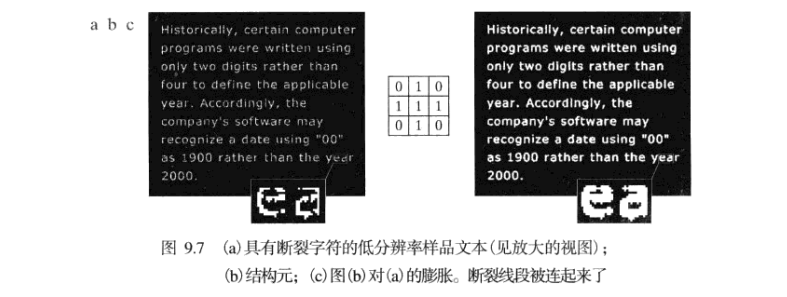
\includegraphics[width=0.9\linewidth]{fig/dilation.png}
\end{figure}

膨胀与腐蚀具有对偶性
\[\begin{aligned}
(A\ominus B)^c &= A^c\oplus B\\
(A\oplus B)^c &= A^c\ominus \hat{B}
\end{aligned}\]

\subsection{开操作与闭操作}
\begin{definition}[开操作]
$B$先对$A$腐蚀,再进行膨胀
\[A\circ B=(A\ominus B)\oplus B=\bigcup\{(B)_z\mid (B)_z\subset A\}\]
实际上就是结构元$B$在$A$内部划过的边界
\begin{figure}[H]
\centering
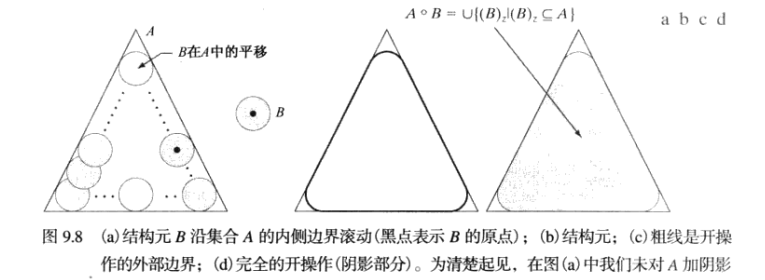
\includegraphics[width=0.9\linewidth]{fig/opening.png}
\end{figure}
\end{definition}
\begin{definition}[闭操作]
$B$先对$A$膨胀,在进行腐蚀
\[A\bullet B=(A\oplus B)\ominus B\]
实际上是结构元$B$在$A$外部划过的边界
\begin{figure}[H]
\centering
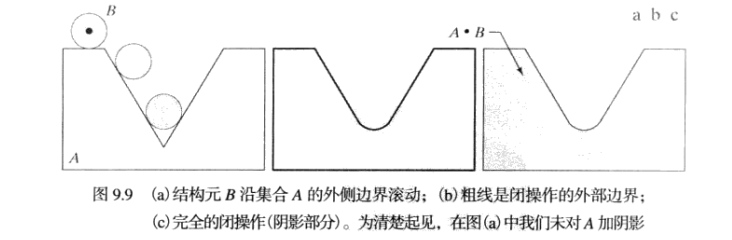
\includegraphics[width=0.9\linewidth]{fig/closing.png}
\end{figure}
\end{definition}

同样,开操作和闭操作也具有对偶性
\[\begin{aligned}
(A\bullet B)^c &= (A^c\circ\hat{B})\\
(A\circ B)^c &= (A^c\bullet\hat{B})
\end{aligned}\]

开操作和闭操作满足
\begin{itemize}
	\item $A\circ B\subset A$,$A\subset A\bullet B$
	\item 若$C\subset D$,则$C\circ B\subset D\circ B$,$C\bullet B\subset D\bullet B$
	\item $(A\circ B)\circ B=A\circ B$,$(A\bullet B)\bullet B=A\bullet B$
\end{itemize}

\subsection{击中或击不中变换}
\begin{definition}[击中或击不中(hit-or-miss)变换]
\[A\circledast B=(A\ominus D)\cap[A^C\ominus(W-D)]=(A\ominus B)\cap(A^C\ominus B_2)\]
\end{definition}
\begin{figure}[H]
\centering
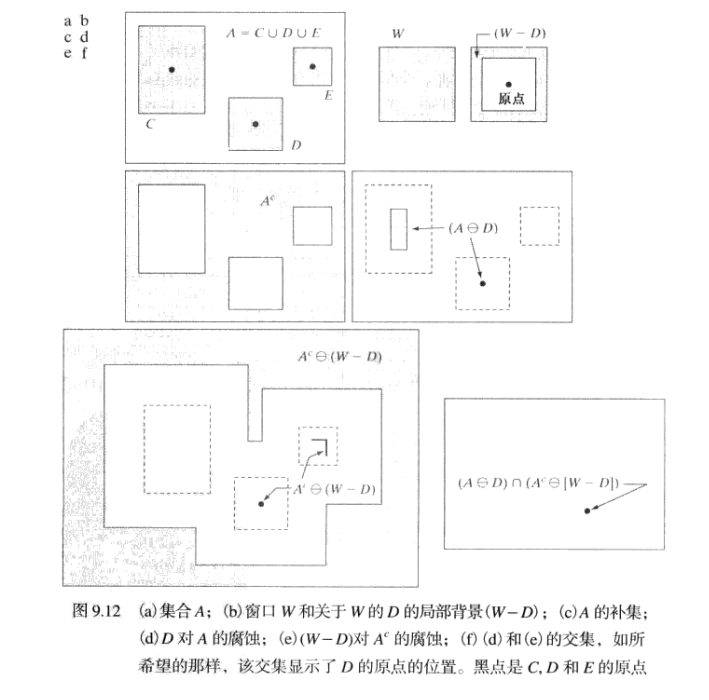
\includegraphics[width=0.9\linewidth]{fig/hit-or-miss.png}
\end{figure}

\subsection{基本形态学算法}
\begin{itemize}
\item 边界提取
\[\beta(A)=A-(A\ominus B)\]
\item 孔洞填充:当$X_k=X_{k-1}$时迭代结束
\[X_k=(X_{k-1}\oplus B)\cap A^C\]
\item 连通分量:当$X_k=X_{k-1}$时迭代结束
\[X_k=(X_{k-1}\oplus B)\cap A\]
\item 凸包/凸壳:令$B^i,i=1,2,3,4$为下列结构元
\begin{figure}[H]
\centering
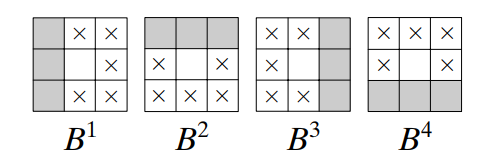
\includegraphics[width=0.4\linewidth]{fig/convex_hull_SE.png}
\end{figure}
\[X_k^i=(X_{k-1}\circledast B^i)\cup A\quad i=1,2,3,4\quad k=1,2,\ldots\]
其中$X_0^i=A$,当该过程收敛$X_k=X_{k-1}^i$时,令$D^i=X_k^i$,则$A$的凸壳为
\[C(A)=\bigcup_{i=1}^4 D^i\]
凸缺为凸包减去原集合
\item 细化
\[A\otimes B=A-(A\circledast B)=A\cap(A\circledast B)^C\]
\item 粗化
\[A\odot B=A\cup (A\circledast B)\]
\item 骨架
\[S(A)=\bigcup_{k=0}^K S_k(A)\]
其中
\[S_k(A)=(A\ominus kB)-(A\ominus kB)\circ B\]
\item 裁剪
\[\begin{aligned}
X_1&=A\otimes \{B\}\\
X_2&=\bigcup_{k=1}^8(X_1\circledast B^k)\\
X_3&=(X_2\oplus H)\cap A\\
X_4&=X_1\cup X_3
\end{aligned}\]
\end{itemize}

\subsection{灰度级形态学}
\begin{definition}[灰度级腐蚀与膨胀]
对非平坦结构元$b_N$的腐蚀
\[[f\ominus b](x,y)=\min_{(s,t)\in b}\{f(x+s,y+t)\}-b_N(s,t)\]
对非平坦结构元$b_N$的膨胀
\[[f\oplus b](x,y)=\max_{(s,t)\in b}\{f(x-s,y-t)\}+b_N(s,t)\]
\end{definition}

开操作与闭操作都有类似的定义及结论。

\begin{definition}[形态学梯度]
\[g=(f\oplus b)-(f\ominus b)\]
\end{definition}

\begin{definition}[顶帽与底帽变换]
顶帽(top-hat)变换
\[T_{hat}(f)=f-(f\circ b)\]
底帽(bottom-hat)变换
\[B_{hat}(f)=(f\bullet b)-f\]
\end{definition}

\begin{figure}[H]
\centering
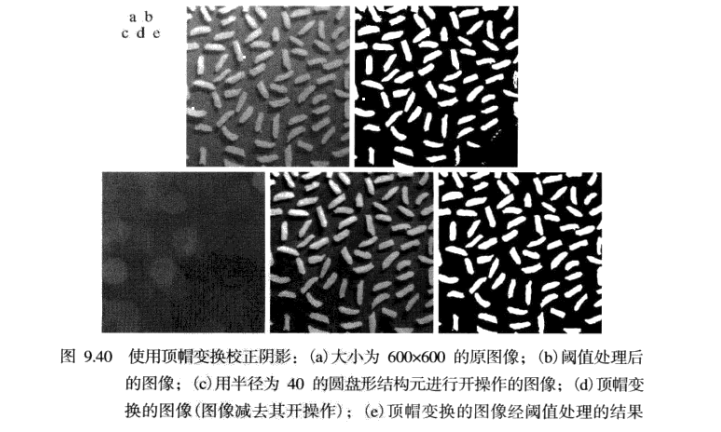
\includegraphics[width=0.8\linewidth]{fig/top-hat.png}
\end{figure}

粒度测定原理:以某一特定的尺度对含有相近尺度颗粒的图像区域进行\textbf{开操作},然后通过计算输
入图像和输出图像之间的差异可以对相近尺寸颗粒的相对数量进行测算。
\begin{figure}[H]
\centering
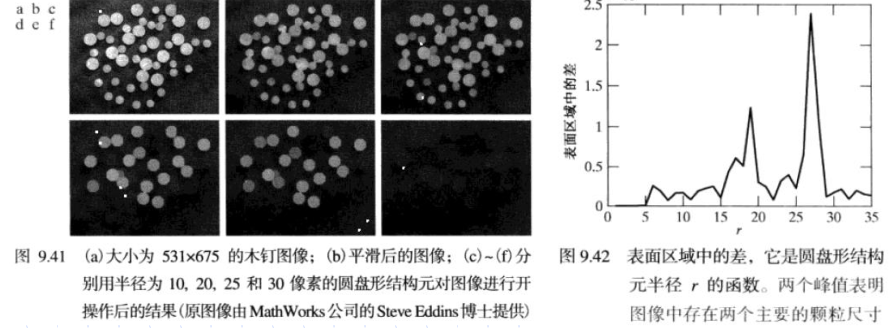
\includegraphics[width=\linewidth]{fig/granulometry.png}
\end{figure}

纹理分割:右边区域的圆点直径比左边大,目的是以纹理为基础找到区域的边界。
算法如下:
\begin{itemize}
\item [(a)] 取尺寸与小斑点大小的结构元素做闭运算(半径30)
\item [(b)] 取比大斑点间隙大的结构元素做开操作(半径60)
\item [(c)] 做二值化(使用全1的$3\times 3$结构元执行梯度画界)
\end{itemize}
\begin{figure}[H]
\centering
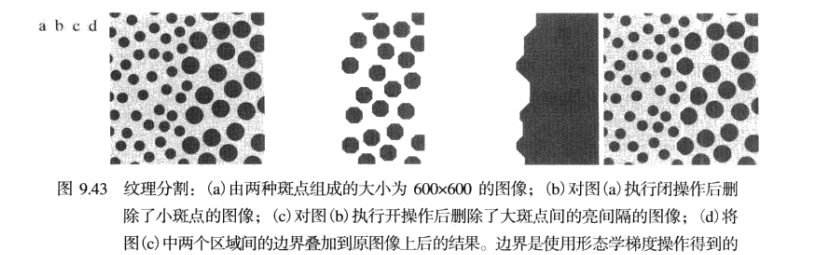
\includegraphics[width=\linewidth]{fig/texture_segment.png}
\end{figure}
% !TEX root = main.tex

\section{图像分割}
图像分割一般基于亮度值的两种基本特性(\textbf{不连续性}和\textbf{相似性})来分割。

\begin{definition}[分割]
令$R$为全图,可将分割看作$R$划分为$n$个子区域$R_1,R_2,\ldots,R_n$的过程:
\begin{enumerate}
	\item $\disp\bigcup_{i=1}^n R_i=R$
	\item $R_i$是一个连通区域
	\item $R_i\cap R_j=\varnothing$
	\item $Q(R_i)=TRUE$
	\item $Q(R_i\cup R_j)=FALSE$,对于任何$R_i$和$R_j$的邻接区域
\end{enumerate}
其中,$Q(R_k)$为定义在集合$R_k$的点上的逻辑属性
\end{definition}

\subsection{点检测与线检测}
\subsubsection{点检测}
\begin{center}
\begin{tabular}{|c|c|c|}\hline
1 & 1 & 1\\\hline
1 & -8 & 1\\\hline
1 & 1 & 1\\\hline
\end{tabular}
\end{center}
若作用算子后的图像$|R(x,y)|\geq T$,则记为$1$。

\subsubsection{线检测}
\begin{figure}[H]
\centering
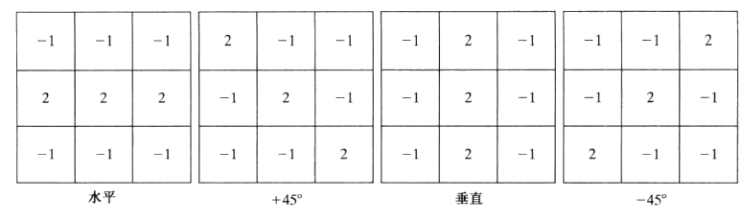
\includegraphics[width=0.9\linewidth]{fig/line_detect.png}
\end{figure}

\subsection{边缘检测}
傅里叶变换无法刻画边缘,只知道高频成分,不知道高频在哪里。
一种方法是局部傅里叶变换,衍生出小波变换(就是要构造一种高通滤波器):有震荡信号的位置(小范围震荡且积分为0),可以刻画边缘。

台阶/阶梯、斜坡/斜、屋顶/Delta边缘模型如下。
\begin{figure}[H]
\centering
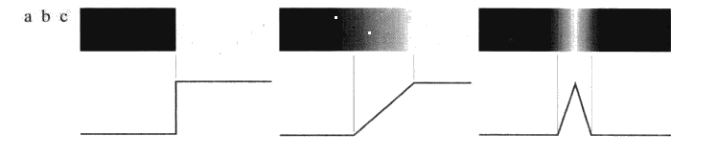
\includegraphics[width=0.9\linewidth]{fig/edge_model.png}
\end{figure}

如下图所示,二阶导数会增大噪声,因此做边缘检测之前应该先抑制噪声(平滑)。
\begin{figure}[H]
\centering
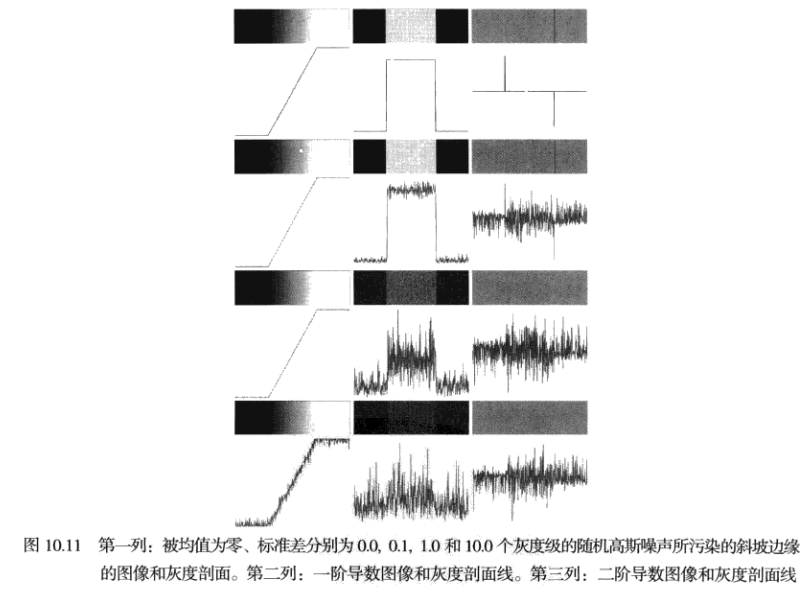
\includegraphics[width=0.9\linewidth]{fig/edge_detect_noise.png}
\end{figure}

常用的边缘检测算子:一阶微分-梯度,二阶微分-Laplace算子
\begin{figure}[H]
\centering
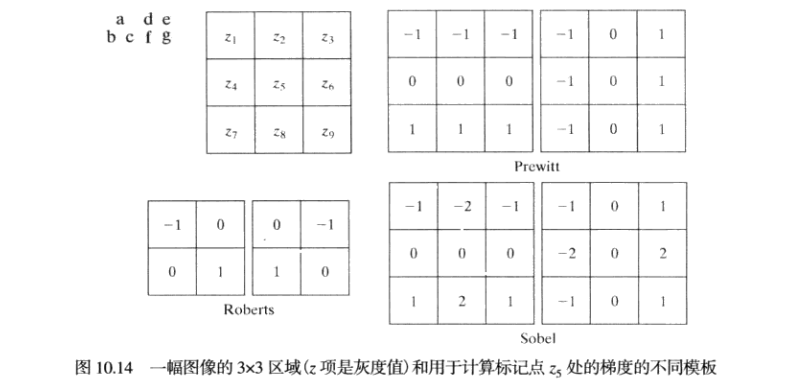
\includegraphics[width=0.9\linewidth]{fig/edge_detect_op.png}
\end{figure}

\subsubsection{Marr-Hildreth边缘检测器}
由于拉普拉斯算子的应用通常会放大图像的噪声,因此通常先平滑,再应用拉普拉斯算子。
假设$f(x,y)$为图像,$h(x,y)$为高斯平滑函数
\[h(x,y)=-\ee^{-\frac{x^2+y^2}{2\sigma^2}}\]
则只需做一步操作完成平滑及边缘检测
\[\nabla^2 [f(x,y)*h(x,y)]=f(x,y)*[\nabla^2 h(x,y)]\]
其中
\[\nabla^2 h(x,y)=\frac{2}{\sigma^2}\lrs{1-\frac{x^2+y^2}{2\sigma^2}}\ee^{-\frac{x^2+y^2}{2\sigma^2}}\]
即高斯拉普拉斯(LoG)变换。

墨西哥草帽函数。
(高斯函数的微分就是一种小波,做微分后负号与负号抵消;而且高斯函数有无穷阶导数)
\begin{figure}[H]
\centering
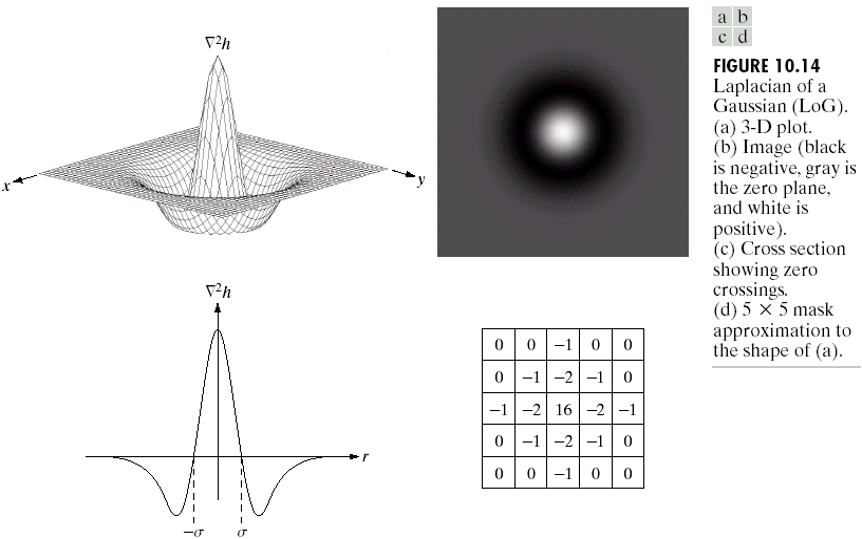
\includegraphics[width=0.6\linewidth]{fig/LoG.png}
\end{figure}

得到Marr-Hildreth的边缘检测算法
\begin{enumerate}
	\item 计算高斯拉普拉斯变换(LoG)
	\item 找到零交叉点(边缘正负变化的地方)
\end{enumerate}

用高斯差分DoG滤波可以近似代替LoG,
\[DoG(x,y)=\frac{1}{2\pi\sigma_1^2}\ee^{-\frac{x^2+y^2}{2\sigma_1^2}}-\frac{1}{2\pi\sigma_2^2}\ee^{-\frac{x^2+y^2}{2\sigma_2^2}},\;\sigma_1>\sigma_2\]
以$\sigma_1:\sigma_2=1.6:1$来定,则近似的$\sigma$为
\[\sigma^2=\frac{\sigma_1^2\sigma_2^2}{\sigma_1^2-\sigma_2^2}\ln\lrs{\frac{\sigma_1^2}{\sigma_2^2}}\]

\subsubsection{Canny边缘检测器}
目标:
\begin{itemize}
	\item 低错误率:边缘一个不落,一个不多
	\item 边缘点应该被很好定位:标记的边缘点与真实边缘中心之间的距离最小
	\item 单一边缘点响应:对于真实的边缘点,检测器仅返回一个点,即真实边缘周围的局部最大数应该最小
\end{itemize}

算法步骤:
\begin{enumerate}
	\item 用一个高斯滤波器平滑输入图像
	\item 计算梯度幅值图像和角度图像(Canny为二阶梯度算子)
	\[M(x,y)=\sqrt{g_x^2+g_y^2},\quad\alpha(x,y)=\arctan\lrs{\frac{g_y}{g_x}}\]
	\item 对梯度幅值图像应用非最大抑制
\begin{figure}[H]
\centering
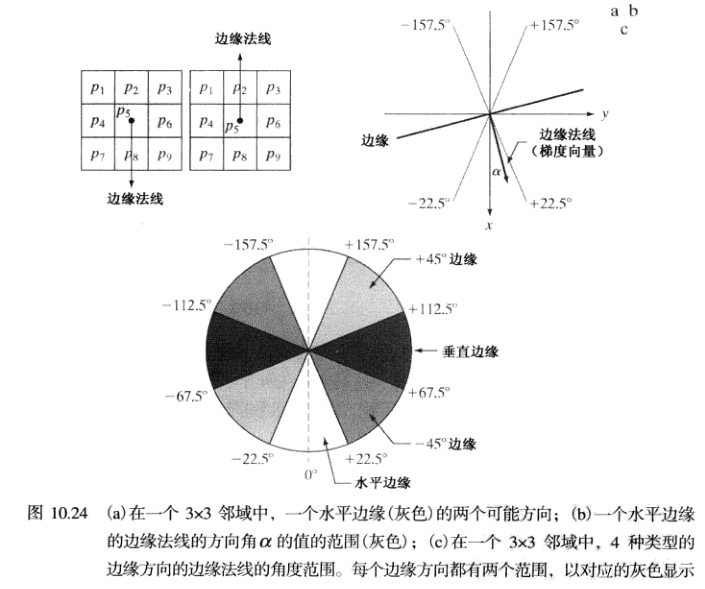
\includegraphics[width=0.6\linewidth]{fig/canny-margin.png}
\end{figure}
\begin{enumerate}
	\item 寻找最接近$\alpha(x,y)$的方向$d$
	\item $g_N$代表细化后的边缘
	\[g_N(x,y)=\begin{cases}0 & M(x,y)\text{的值至少小于沿$d$的两个邻居之一}\\M(x,y) & \text{否则}\end{cases}\]
\end{enumerate}
	\item 用双阈值处理和连接分析来检测并连接边缘\\
	双阈值法:高阈值$T_H$和低阈值$T_L$,比率为$2:1$或$3:1$
	\[\begin{aligned}
	g_{NN}(x,y) &= g_N(x,y)\geq T_H & \text{强边缘}\\
	g_{NL}(x,y) &= g_N(x,y)\geq T_L & \text{弱边缘(可能是边缘也可能不是)+强边缘}\\
	g_{NL}(x,y) &= g_{NL}(x,y)-g_{NH}(x,y) & \text{弱边缘}
	\end{aligned}\]
	用弱边缘补齐强边缘来获得完整边缘
\begin{enumerate}
	\item 在$g_{NN}(x,y)$中定位下一个未被访问的边缘像素$p$
	\item 在$g_{NL}(x,y)$中用8连通方法连接到$p$
	\item 如果$g_{NN}(x,y)$中所有非零标记都已经访问过,则跳到(d),否则(a)
	\item 将$g_{NL}(x,y)$中未被标记为有效边缘的像素的所有像素置零。
	将$g_{NL}(x,y)$中非零像素附加到$g_{NN}(x,y)$
\end{enumerate}
\end{enumerate}

\subsection{边缘连接}
\textbf{边界是封闭的边缘。}
\[\text{边界检测}=\text{边缘检测}+\text{边缘连接}\]

\begin{itemize}
\item 边缘连接:两个端点只有在边缘强度和走向相近的情况下才能连接。
如果像素$(s,t)$在像素$(x,y)$的邻域内且满足:
\[|M(x,y)-M(s,t)|\leq E,\quad |\alpha(x,y)-\alpha(s,t)|\leq A\]
则可以将$(s,t)$与$(x,y)$连接起来。

\item 边界跟踪:依照角度搜索,用$3\times 3$区域平均值代替单像素点(避免噪声影响),称为虫
\begin{figure}[H]
\centering
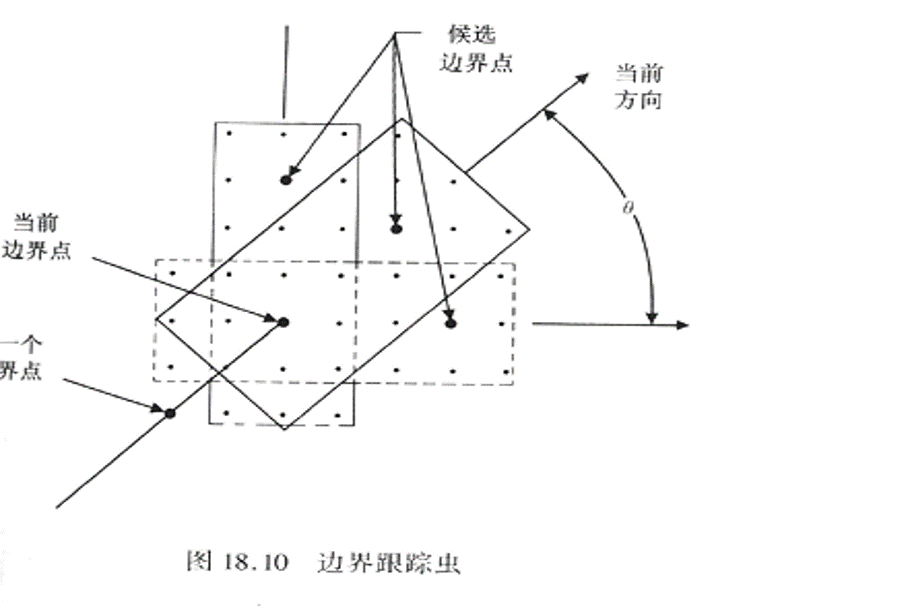
\includegraphics[width=0.5\linewidth]{fig/boundary_tracing.png}
\end{figure}

\item 区域处理:用多边形拟合算法
\begin{figure}[H]
\centering
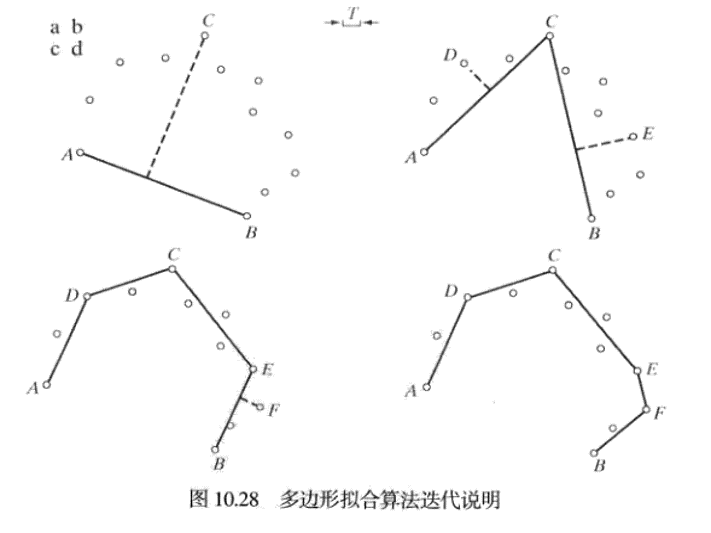
\includegraphics[width=0.5\linewidth]{fig/polygon_boundary.png}
\end{figure}
\end{itemize}

\subsection{边界检测}
用Hough变换进行边界检测:通过边界点找已知形状的目标。 % 考试必考

\subsubsection{直线检测问题}
已知一组边缘点,找一条直线,使它通过最多边缘点。

直线方程用极坐标表示
\[\rho=x\cos\theta+y\sin\theta\]
通过辅助角变换可得
\[\rho=A_0\sin(\theta+\phi_0)\]
故可映射到$\rho O\theta$空间,其中每一个点是$xOy$平面上的通过同一个点的一条线。
\begin{figure}[H]
\centering
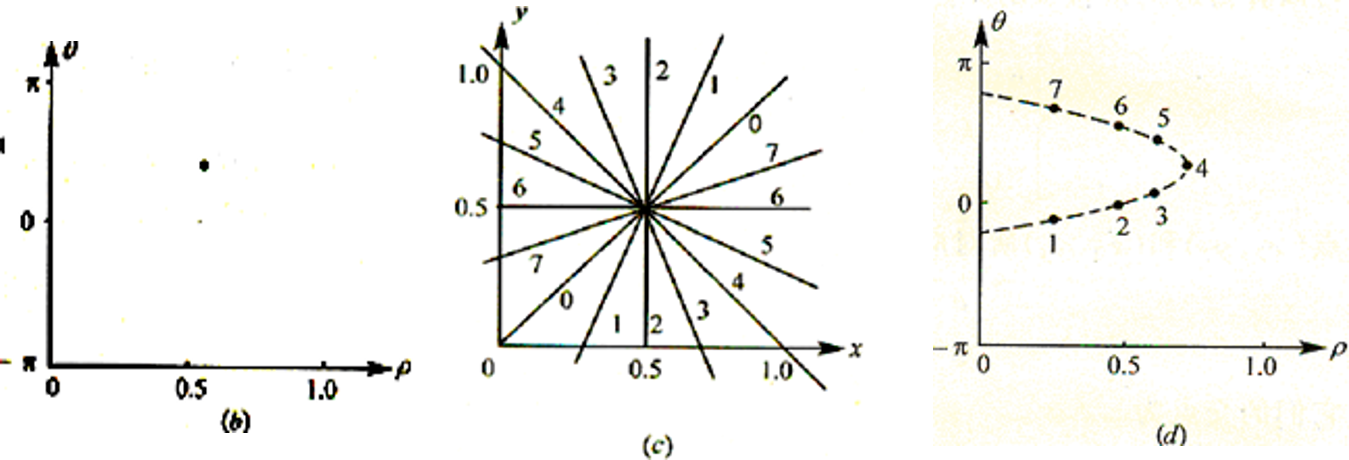
\includegraphics[width=0.6\linewidth]{fig/hough.png}
\end{figure}

如果有一组位于由参数$\rho_0$和$\theta_0$决定的直线上的边缘点,则每个边缘点对应了$\rho,\theta$空间的一条正弦曲线。
所有这些曲线必然会交于点$(\rho_0,\theta_0)$,因为这是它们共享的一条直线的参数。
\begin{figure}[H]
\centering
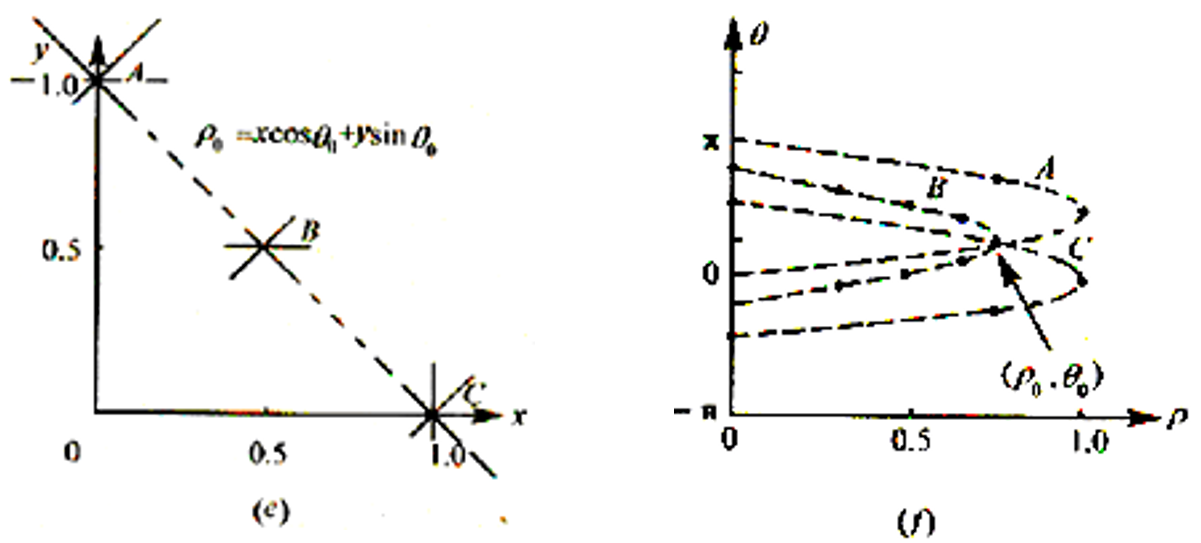
\includegraphics[width=0.6\linewidth]{fig/hough2.png}
\end{figure}

故对于边缘点的直线拟合问题,即找一个使边缘点确定的正弦曲线相交最多的点$(\rho,\theta)$。

可以建立$\rho,\theta$空间的二维直方图来确定对于边缘点的最佳拟合直线参数$(\rho_0,\theta_0)$。
具体算法如下:
\begin{enumerate}
	\item 对于每个边缘点$(x,y)$。建立直线方程:
	\[\rho=x\cos(\theta)+y\sin(\theta)\]
	\item 假定$\rho,\theta$的变化范围为$\rho\in[\rho_{\min},\rho_{\max}],\theta\in[\theta_{\min},\theta_{\max}]$,建立$A(\rho,\theta)$累加器
	\item 给定$\theta$,由原始方程确定$\rho$,则$A(\rho,\theta)+=1$
	\item 对于所有的边缘点,执行上述步骤,找出最大的$A(\rho,\theta)$,即为所求
\end{enumerate}

\subsubsection{其他检测问题}
换成圆/椭圆也一样
\[(x-x_0)^2+(y-y_0)^2=r^2\]
在参数空间建立3D累加数组$A$,让$(x_0,y_0)$变化,计算$r$。


\subsection{阈值处理}
阈值处理模型
\[T=T[x,y,p(x,y),f(x,y)\]
如果
\[g(x,y)=\begin{cases}
1 & f(x,y)>T\\
0 & f(x,y)\leq T
\end{cases}\]
当$T$为适用于整个图像的常数时,则该公式给出的处理为全局阈值处理,$f(x,y)>T$的任何点为一个对象点,否则该点为背景点。
如果取决于邻域$p(x,y)$,则为局部阈值处理。
如果取决于$(x,y)$本身,则为动态阈值处理/自适应阈值处理。

背景光照不均匀时阈值处理方法:
\begin{enumerate}
	\item 直接矫正方法:用恒定灰度的平坦表面成像获得光照模式,用相反的模式与图像相乘来矫正
	\item 采用顶帽变换来获得全局阴影模式
	\item 使用可变阈值近似处理非均匀性
\end{enumerate}

\subsubsection{基本全局阈值处理}
试探法:
\begin{enumerate}
	\item 为全局阈值$T$选择一个初始估计值
	\item 用$T$分割图像,生成两组像素:$G_1$由所有灰度值大于$T$的像素组成,而$G_2$   由所有灰度值小于或等于$T$的像素组成。
	\item 对区域$G_1$和$G_2$中的所有像素计算平均灰度值$m_1$和$m_2$
	\item 计算新的门限值:$T=1/2(m_1+m_2)$
	\item 重复步骤2到4,直到逐次迭代所得的$T$值之差小于实现定义的参数$\Delta T$
\end{enumerate}

\subsubsection{Otsu最佳全局阈值处理}
将其看为一个分类问题,用贝叶斯决策。

\begin{enumerate}
\item 归一化直方图$p_i=n_i/(NM)$
\item 给定阈值$T(k)$,将其分为左右两个部分$C_1$和$C_2$
\item 求出两块的条件概率密度$p_i/P_1(k)$和$p_i/P_2(k)$
\item 定义归一化度量指标$\eta=\frac{\sigma_B^2}{\sigma_G^2}$\\
其中$\sigma_G^2$为全局方差
\[\sigma_G^2=\sum_{i=0}^{L-1}(i-m_G)^2p_i\]
$\sigma_B^2$为类间方差
\[\begin{aligned}
\sigma_B^2 &= P_1(m_1-m_G)^2+P_2(m_2-m_G)^2\\
&=P_1P_2(m_1-m_2)^2\\
&=\frac{(m_G P_1-m)^2}{P_1(1-P_1)}
\end{aligned}\]
\item 基本结论是$m_1$和$m_2$相隔越大,则$\sigma_B^2$越大;$\eta$是分割的可分性度量,$\sigma_B^2$越大,则$\eta$越大。
进而有最佳阈值
\[\sigma_B^2(k^*)=\max_{0\leq k\leq L-1}\sigma_B^2(k)\]
\end{enumerate}

\subsubsection{预处理}
用图像平滑来改善全局阈值处理:但难以处理单峰

用边缘来改进全局阈值处理:梯度算法能能够区分边缘区域与平坦区域;拉普拉斯算子可以确定给定的像素在边缘的亮一边还是暗一边。
局部阈值法:
\[s(x,y)=\begin{cases}
0 & \nabla f<T\\
+ & \nabla f\geq T, \nabla^2 f\geq 0\\
- & \nabla f\geq T, \nabla^2 f< 0
\end{cases}\]
\begin{enumerate}
	\item 计算$f(x,y)$的梯度图或者拉普拉斯绝对值图
	\item 给定一个阈值
	\item 用步骤2)的阈值对步骤1)的结果做阈值处理(通常取第$n$个百分比),产生二值图像$g_T(x,y)$(可以是梯度二值图和拉普拉斯绝对值图二值图取“或”的组合)
	\item 计算$h(x,y)=f(x,y).*g_T(x,y)$,计算$h(x,y)$的直方图
	\item 在4)直方图的基础上,用Otsu方法做图像分割
\end{enumerate}

\subsubsection{多阈值处理}
在$K$个类的情况下,同样可以定义类间方差,来计算最大的归一化度量指标

\subsubsection{可变阈值处理}
通过图像分块的阈值处理,因为块内的光照近似均匀


\subsection{基于区域的分割}
$f(x,y)$为图像,$S(x,y)$为种子阵列,种子处为1,其他为0。
$Q$为位置$(x,y)$的属性,基于8连通的区域生长算法为:
\begin{enumerate}
	\item 在$S(x,y)$中找连通分量,并将连通分量腐蚀为一个像素;
	将找到的所有这种像素标记为$1$,$S$的其他像素标记为$0$
	\item 计算
	\[f_Q(x,y)=\begin{cases}
	1 & \text{$(x,y)$处属性$Q$为真}\\
	0 & \text{其他}
	\end{cases}\]
	\item 分割后图像$g$为:把$f_Q$中与种子点8连通的所有1值点添加到$S$中的每个种子点
	\item 使用不同的区域标记出$g$中的每个连通分量
\end{enumerate}

\begin{itemize}
	\item 区域生长法
	\item 区域分离合并法
\end{itemize}

\end{document}